%%=============================================================================
%% LaTeX sjabloon voor bachelorproef, HoGent Bedrijf en Organisatie
%% Opleiding Toegepaste Informatica
%%=============================================================================

\documentclass[fleqn,a4paper,12pt]{book}

%%=============================================================================
%% LaTeX sjabloon voor de bachelorproef, HoGent Bedrijf en Organisatie
%% Opleiding toegepaste informatica
%%
%% Structuur en algemene vormgeving. Meestal hoef je hier niets te wijzigen.
%%
%% Vormgeving gebaseerd op "The Legrand Orange Book", version 2.0 (9/2/15)
%% door Mathias Legrand (legrand.mathias@gmail.com) met aanpassingen door
%% Vel (vel@latextemplates.com). Het oorspronkelijke template is te vinden op
%% http://www.LaTeXTemplates.com
%%
%% Aanpassingen voor HoGent toegepaste informatica: 
%%   Bert Van Vreckem <bert.vanvreckem@hogent.be>
%% Licentie: 
%%   CC BY-NC-SA 3.0 (http://creativecommons.org/licenses/by-nc-sa/3.0/)
%%=============================================================================

%%-----------------------------------------------------------------------------
%% Packages
%%-----------------------------------------------------------------------------

\usepackage[top=3cm,bottom=3cm,left=3cm,right=3cm,headsep=10pt,a4paper]{geometry} % Page margins
\usepackage[utf8]{inputenc}  % Accenten gebruiken in tekst (vb. é ipv \'e)
\usepackage{amsfonts}        % AMS math packages: extra wiskundige
\usepackage{amsmath}         %   symbolen (o.a. getallen-
\usepackage{amssymb}         %   verzamelingen N, R, Z, Q, etc.)
\usepackage[english,dutch]{babel}    % Taalinstellingen: woordsplitsingen,
                             %  commando's voor speciale karakters
                             %  ("dutch" voor NL)
\usepackage{iflang}
\usepackage{eurosym}         % Euro-symbool €
\usepackage{geometry}
\usepackage{graphicx}        % Invoegen van tekeningen
\graphicspath{{img/}}       % Specifies the directory where pictures are stored
\usepackage{tikz}            % Required for drawing custom shapes
\usepackage[pdftex,bookmarks=true]{hyperref}
                             % PDF krijgt klikbare links & verwijzingen,
                             %  inhoudstafel
\usepackage{enumitem}        % Customize lists
\setlist{nolistsep}         % Reduce spacing between list items
\usepackage{listings}        % Broncode mooi opmaken
\usepackage{multirow}        % Tekst over verschillende cellen in tabellen
\usepackage{rotating}        % Tabellen en figuren roteren

\usepackage{booktabs}        % Required for nicer horizontal rules in tables

\usepackage{xcolor}          % Required for specifying colors by name
\definecolor{maincolor}{RGB}{0,147,208} % Define the main color used for 
                             % highlighting throughout the book
                             % 0, 147, 208 = officiële kleur HoGent FBO

% Paragraph style: no indent, add space between paragraphs
\setlength{\parindent}{0em}
\setlength{\parskip}{1em}

\usepackage{etoolbox}
\usepackage{titling} % Macros for title, author, etc
\usepackage{lipsum}          % Voor vultekst (lorem ipsum)

%----------------------------------------------------------------------------------------
%	FONTS
%----------------------------------------------------------------------------------------

\usepackage{avant} % Use the Avantgarde font for headings
%\usepackage{times} % Use the Times font for headings
\usepackage{mathptmx} % Use the Adobe Times Roman as the default text font together with math symbols from the Sym­bol, Chancery and Com­puter Modern fonts

\usepackage{microtype} % Slightly tweak font spacing for aesthetics
\usepackage[utf8]{inputenc} % Required for including letters with accents
\usepackage[T1]{fontenc} % Use 8-bit encoding that has 256 glyphs

%------------------------------------------------------------------------------
%	TITLE PAGE
%------------------------------------------------------------------------------

\newcommand{\inserttitlepage}{%
\begin{titlepage}
  \newgeometry{top=2cm,bottom=1.5cm,left=1.5cm,right=1.5cm}
  \begin{center}

    \begingroup
    \rmfamily
    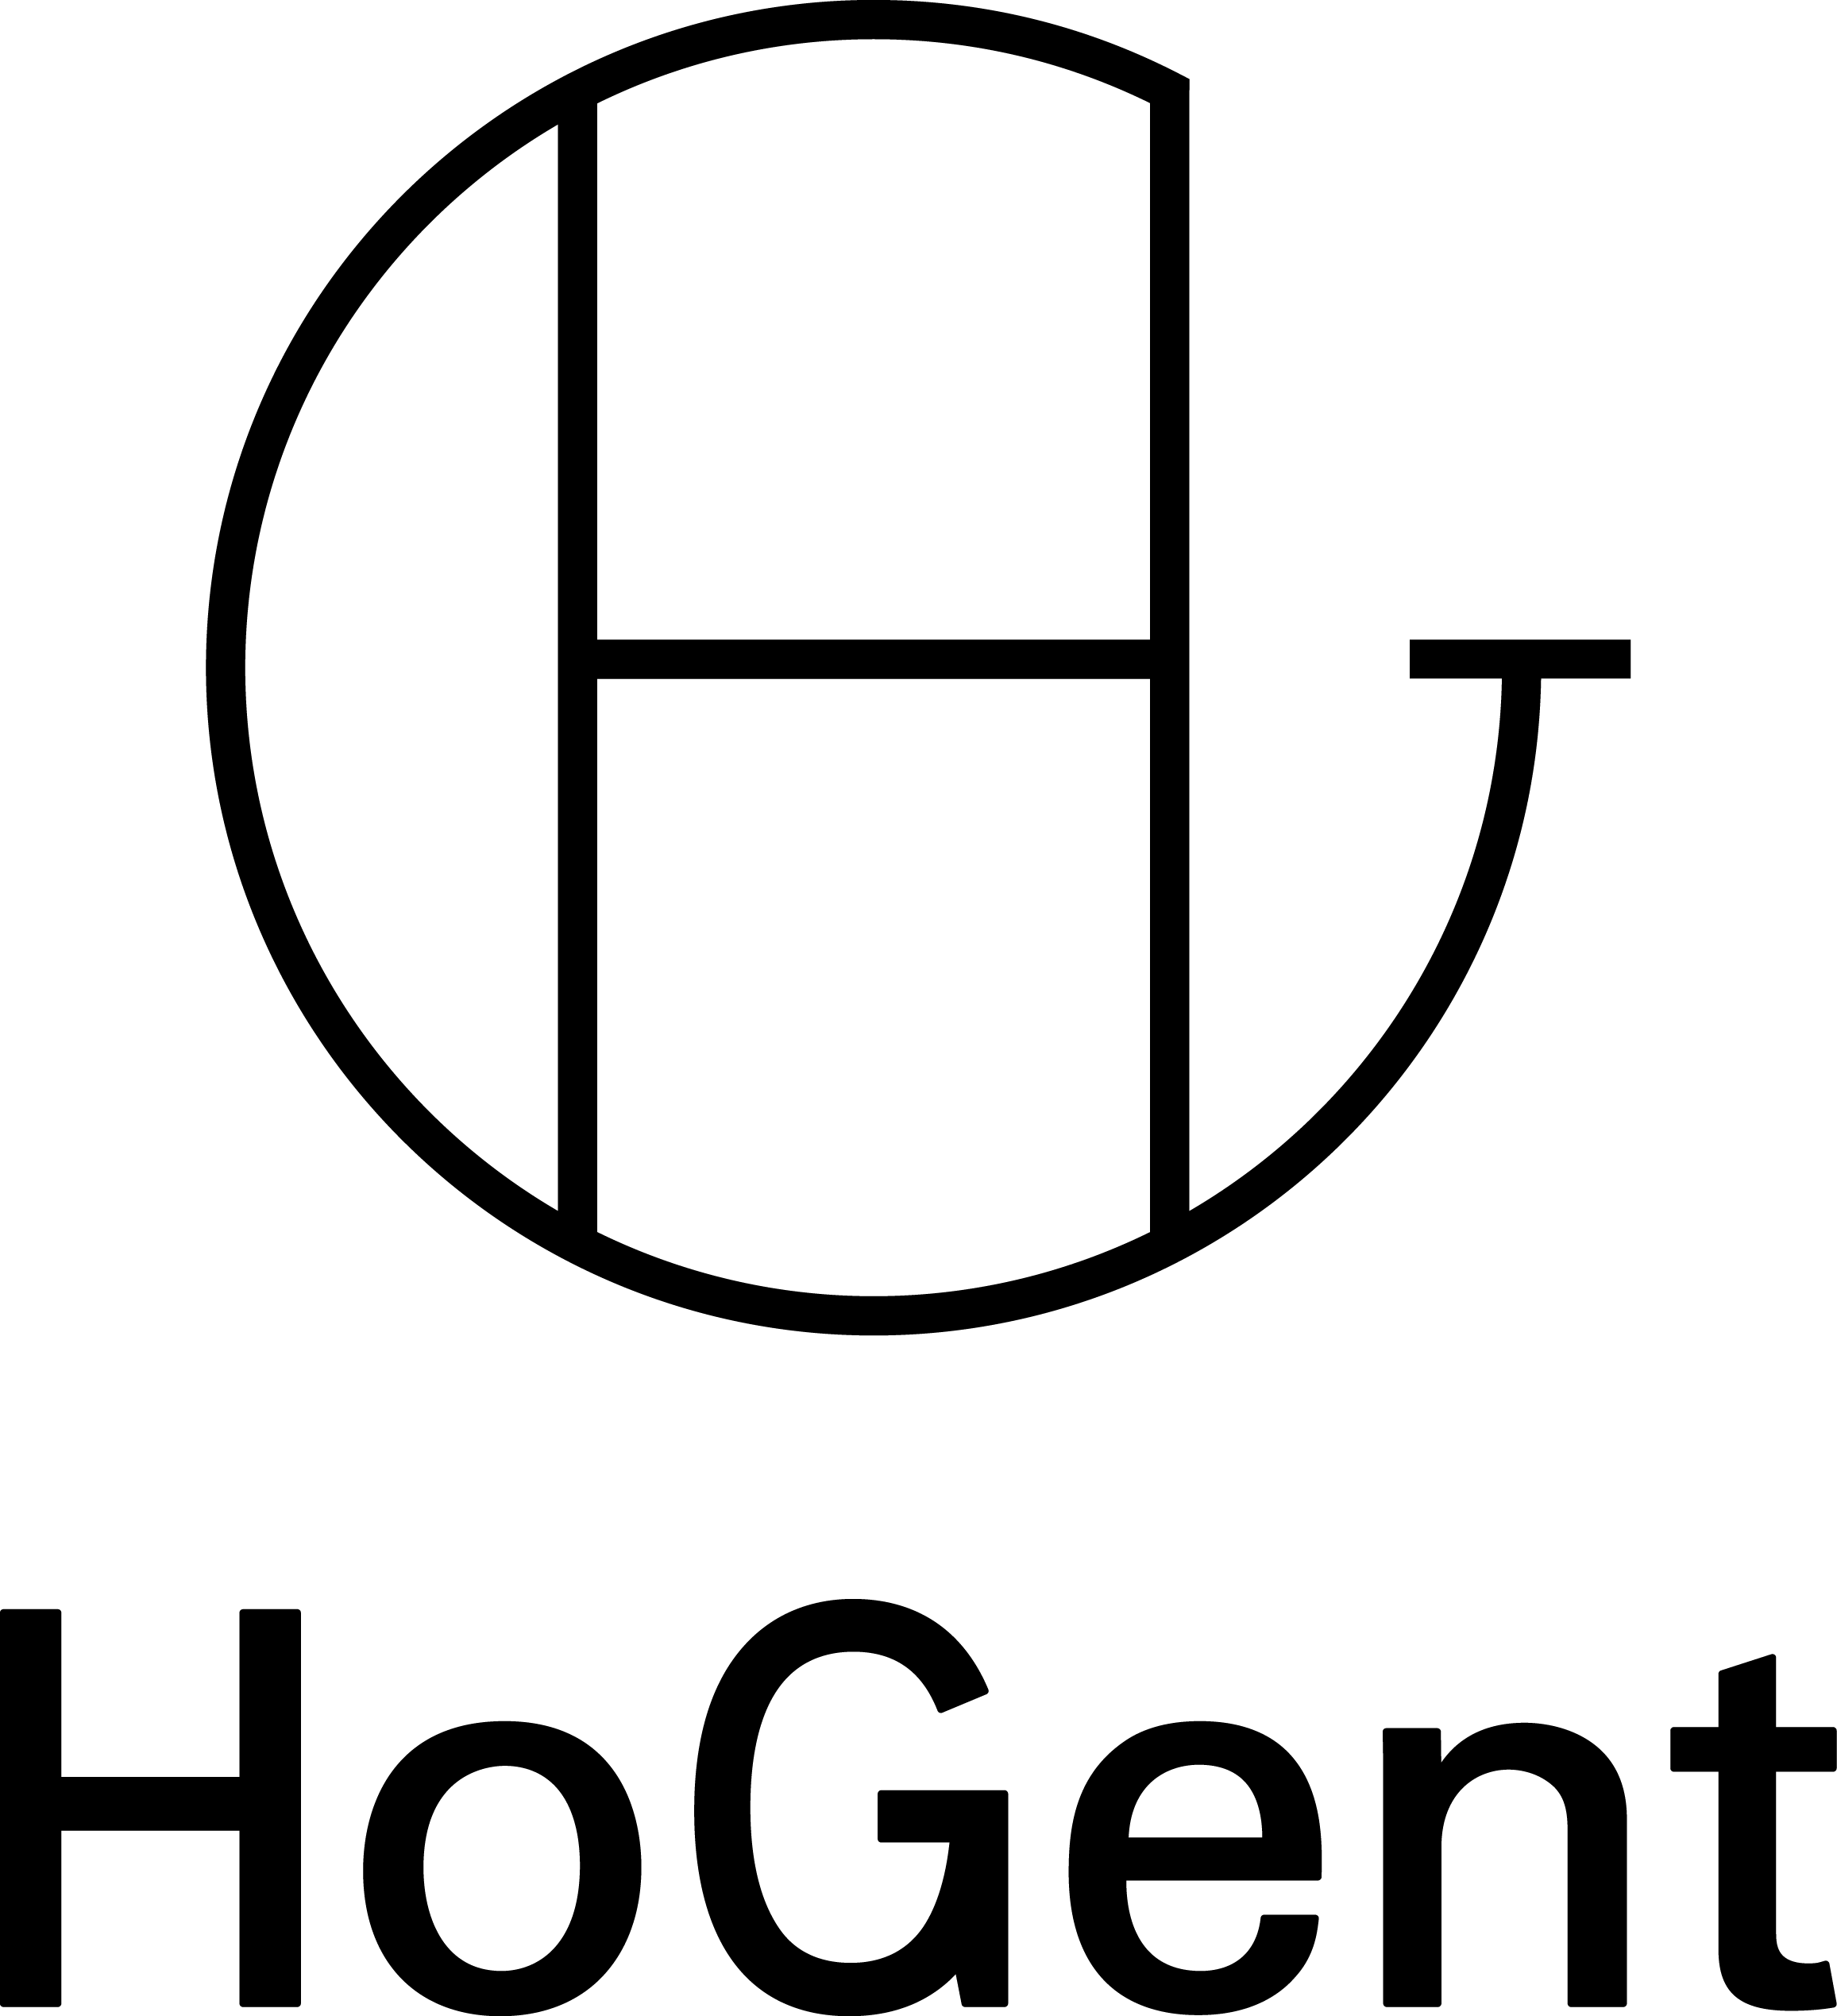
\includegraphics[width=2.5cm]{img/HG-beeldmerk-woordmerk}\\[.5cm]
    Faculteit Bedrijf en Organisatie\\[3cm]
    \titel
    \vfill
    \student\\[3.5cm]
    Scriptie voorgedragen tot het bekomen van de graad van\\professionele bachelor in de toegepaste informatica\\[2cm]
    Promotor:\\
    \promotor\\
    \ifdefempty{\copromotor}{\vspace{2.5cm}}{Co-promotor:\\\copromotor\\[2.5cm]}
    Instelling: \instelling\\[.5cm]
    Academiejaar: \academiejaar\\[.5cm]
    \ifcase \examenperiode \or Eerste \or Tweede \else Derde \fi examenperiode
    \endgroup

  \end{center}
  \restoregeometry
\end{titlepage}
  \emptypage
\begin{titlepage}
  \newgeometry{top=5.35cm,bottom=1.5cm,left=1.5cm,right=1.5cm}
  \begin{center}

    \begingroup
    \rmfamily
    \IfLanguageName{dutch}{Faculteit Bedrijf en Organisatie}{Faculty of Business and Information Management}\\[3cm]
    \titel
    \vfill
    \student\\[3.5cm]
    \IfLanguageName{dutch}{Scriptie voorgedragen tot het bekomen van de graad van\\professionele bachelor in de toegepaste informatica}{Thesis submitted in partial fulfilment of the requirements for the degree of\\professional bachelor of applied computer science}\\[2cm]
    Promotor:\\
    \promotor\\
    \ifdefempty{\copromotor}{\vspace{2.5cm}}{Co-promotor:\\\copromotor\\[2.5cm]}
    \IfLanguageName{dutch}{Instelling}{Institution}: \instelling\\[.5cm]
    \IfLanguageName{dutch}{Academiejaar}{Academic year}: \academiejaar\\[.5cm]
    \IfLanguageName{dutch}{%
    \ifcase \examenperiode \or Eerste \or Tweede \else Derde \fi examenperiode}{%
    \ifcase \examenperiode \or First \or Second \else Third \fi examination period}
    \endgroup

  \end{center}
  \restoregeometry
\end{titlepage}
}

%----------------------------------------------------------------------------------------
%	BIBLIOGRAPHY AND INDEX
%----------------------------------------------------------------------------------------

\usepackage[style=apa,backend=biber]{biblatex}
\usepackage{csquotes}
\DeclareLanguageMapping{dutch}{dutch-apa}
\addbibresource{bachproef-tin.bib} % BibTeX bibliography file
\addbibresource{../voorstel/voorstel.bib}
\defbibheading{bibempty}{}

\usepackage{calc} % For simpler calculation - used for spacing the index letter headings correctly
\usepackage{makeidx} % Required to make an index
\makeindex % Tells LaTeX to create the files required for indexing

%----------------------------------------------------------------------------------------
%	MAIN TABLE OF CONTENTS
%----------------------------------------------------------------------------------------

\usepackage{titletoc} % Required for manipulating the table of contents

\contentsmargin{0cm} % Removes the default margin

% Part text styling
\titlecontents{part}[0cm]
{\addvspace{20pt}\centering\large\bfseries}
{}
{}
{}

% Chapter text styling
\titlecontents{chapter}[1.25cm] % Indentation
{\addvspace{12pt}\large\sffamily\bfseries} % Spacing and font options for chapters
{\color{maincolor!60}\contentslabel[\Large\thecontentslabel]{1.25cm}\color{maincolor}} % Chapter number
{\color{maincolor}}
{\color{maincolor!60}\normalsize\;\titlerule*[.5pc]{.}\;\thecontentspage} % Page number

% Section text styling
\titlecontents{section}[1.25cm] % Indentation
{\addvspace{3pt}\sffamily\bfseries} % Spacing and font options for sections
{\contentslabel[\thecontentslabel]{1.25cm}} % Section number
{}
{\hfill\color{black}\thecontentspage} % Page number
[]

% Subsection text styling
\titlecontents{subsection}[1.25cm] % Indentation
{\addvspace{1pt}\sffamily\small} % Spacing and font options for subsections
{\contentslabel[\thecontentslabel]{1.25cm}} % Subsection number
{}
{\ \titlerule*[.5pc]{.}\;\thecontentspage} % Page number
[]

% List of figures
\titlecontents{figure}[0em]
{\addvspace{-5pt}\sffamily}
{\thecontentslabel\hspace*{1em}}
{}
{\ \titlerule*[.5pc]{.}\;\thecontentspage}
[]

% List of tables
\titlecontents{table}[0em]
{\addvspace{-5pt}\sffamily}
{\thecontentslabel\hspace*{1em}}
{}
{\ \titlerule*[.5pc]{.}\;\thecontentspage}
[]

%----------------------------------------------------------------------------------------
%	MINI TABLE OF CONTENTS IN PART HEADS
%----------------------------------------------------------------------------------------

% Chapter text styling
\titlecontents{lchapter}[0em] % Indenting
{\addvspace{15pt}\large\sffamily\bfseries} % Spacing and font options for chapters
{\color{maincolor}\contentslabel[\Large\thecontentslabel]{1.25cm}\color{maincolor}} % Chapter number
{}
{\color{maincolor}\normalsize\sffamily\bfseries\;\titlerule*[.5pc]{.}\;\thecontentspage} % Page number

% Section text styling
\titlecontents{lsection}[0em] % Indenting
{\sffamily\small} % Spacing and font options for sections
{\contentslabel[\thecontentslabel]{1.25cm}} % Section number
{}
{}

% Subsection text styling
\titlecontents{lsubsection}[.5em] % Indentation
{\normalfont\footnotesize\sffamily} % Font settings
{}
{}
{}

%----------------------------------------------------------------------------------------
%	PAGE HEADERS
%----------------------------------------------------------------------------------------

\usepackage{fancyhdr} % Required for header and footer configuration

\pagestyle{fancy}
\renewcommand{\chaptermark}[1]{\markboth{\sffamily\normalsize\bfseries\chaptername\ \thechapter.\ #1}{}} % Chapter text font settings
\renewcommand{\sectionmark}[1]{\markright{\sffamily\normalsize\thesection\hspace{5pt}#1}{}} % Section text font settings
\fancyhf{} \fancyhead[LE,RO]{\sffamily\normalsize\thepage} % Font setting for the page number in the header
\fancyhead[LO]{\rightmark} % Print the nearest section name on the left side of odd pages
\fancyhead[RE]{\leftmark} % Print the current chapter name on the right side of even pages
\renewcommand{\headrulewidth}{0.5pt} % Width of the rule under the header
\addtolength{\headheight}{2.5pt} % Increase the spacing around the header slightly
\renewcommand{\footrulewidth}{0pt} % Removes the rule in the footer
\fancypagestyle{plain}{\fancyhead{}\renewcommand{\headrulewidth}{0pt}} % Style for when a plain pagestyle is specified

% Removes the header from odd empty pages at the end of chapters
\makeatletter
\renewcommand{\cleardoublepage}{
\clearpage\ifodd\c@page\else
\hbox{}
\vspace*{\fill}
\thispagestyle{empty}
\newpage
\fi}

%----------------------------------------------------------------------------------------
%	THEOREM STYLES
%----------------------------------------------------------------------------------------

\usepackage{amsmath,amsfonts,amssymb,amsthm} % For math equations, theorems, symbols, etc

\newcommand{\intoo}[2]{\mathopen{]}#1\,;#2\mathclose{[}}
\newcommand{\ud}{\mathop{\mathrm{{}d}}\mathopen{}}
\newcommand{\intff}[2]{\mathopen{[}#1\,;#2\mathclose{]}}
\newtheorem{notation}{Notation}[chapter]

% Boxed/framed environments
\newtheoremstyle{maincolornumbox}% % Theorem style name
{0pt}% Space above
{0pt}% Space below
{\normalfont}% % Body font
{}% Indent amount
{\small\bf\sffamily\color{maincolor}}% % Theorem head font
{\;}% Punctuation after theorem head
{0.25em}% Space after theorem head
{\small\sffamily\color{maincolor}\thmname{#1}\nobreakspace\thmnumber{\@ifnotempty{#1}{}\@upn{#2}}% Theorem text (e.g. Theorem 2.1)
\thmnote{\nobreakspace\the\thm@notefont\sffamily\bfseries\color{black}---\nobreakspace#3.}} % Optional theorem note
\renewcommand{\qedsymbol}{$\blacksquare$}% Optional qed square

\newtheoremstyle{blacknumex}% Theorem style name
{5pt}% Space above
{5pt}% Space below
{\normalfont}% Body font
{} % Indent amount
{\small\bf\sffamily}% Theorem head font
{\;}% Punctuation after theorem head
{0.25em}% Space after theorem head
{\small\sffamily{\tiny\ensuremath{\blacksquare}}\nobreakspace\thmname{#1}\nobreakspace\thmnumber{\@ifnotempty{#1}{}\@upn{#2}}% Theorem text (e.g. Theorem 2.1)
\thmnote{\nobreakspace\the\thm@notefont\sffamily\bfseries---\nobreakspace#3.}}% Optional theorem note

\newtheoremstyle{blacknumbox} % Theorem style name
{0pt}% Space above
{0pt}% Space below
{\normalfont}% Body font
{}% Indent amount
{\small\bf\sffamily}% Theorem head font
{\;}% Punctuation after theorem head
{0.25em}% Space after theorem head
{\small\sffamily\thmname{#1}\nobreakspace\thmnumber{\@ifnotempty{#1}{}\@upn{#2}}% Theorem text (e.g. Theorem 2.1)
\thmnote{\nobreakspace\the\thm@notefont\sffamily\bfseries---\nobreakspace#3.}}% Optional theorem note

% Non-boxed/non-framed environments
\newtheoremstyle{maincolornum}% % Theorem style name
{5pt}% Space above
{5pt}% Space below
{\normalfont}% % Body font
{}% Indent amount
{\small\bf\sffamily\color{maincolor}}% % Theorem head font
{\;}% Punctuation after theorem head
{0.25em}% Space after theorem head
{\small\sffamily\color{maincolor}\thmname{#1}\nobreakspace\thmnumber{\@ifnotempty{#1}{}\@upn{#2}}% Theorem text (e.g. Theorem 2.1)
\thmnote{\nobreakspace\the\thm@notefont\sffamily\bfseries\color{black}---\nobreakspace#3.}} % Optional theorem note
\renewcommand{\qedsymbol}{$\blacksquare$}% Optional qed square
\makeatother

% Defines the theorem text style for each type of theorem to one of the three styles above
\newcounter{dummy}
\numberwithin{dummy}{section}
\theoremstyle{maincolornumbox}
\newtheorem{theoremeT}[dummy]{Theorem}
\newtheorem{problem}{Problem}[chapter]
\newtheorem{exerciseT}{Exercise}[chapter]
\theoremstyle{blacknumex}
\newtheorem{exampleT}{Example}[chapter]
\theoremstyle{blacknumbox}
\newtheorem{vocabulary}{Vocabulary}[chapter]
\newtheorem{definitionT}{Definition}[section]
\newtheorem{corollaryT}[dummy]{Corollary}
\theoremstyle{maincolornum}
\newtheorem{proposition}[dummy]{Proposition}

%----------------------------------------------------------------------------------------
%	DEFINITION OF COLORED BOXES
%----------------------------------------------------------------------------------------

\RequirePackage[framemethod=default]{mdframed} % Required for creating the theorem, definition, exercise and corollary boxes

% Theorem box
\newmdenv[skipabove=7pt,
skipbelow=7pt,
backgroundcolor=black!5,
linecolor=maincolor,
innerleftmargin=5pt,
innerrightmargin=5pt,
innertopmargin=5pt,
leftmargin=0cm,
rightmargin=0cm,
innerbottommargin=5pt]{tBox}

% Exercise box
\newmdenv[skipabove=7pt,
skipbelow=7pt,
rightline=false,
leftline=true,
topline=false,
bottomline=false,
backgroundcolor=maincolor!10,
linecolor=maincolor,
innerleftmargin=5pt,
innerrightmargin=5pt,
innertopmargin=5pt,
innerbottommargin=5pt,
leftmargin=0cm,
rightmargin=0cm,
linewidth=4pt]{eBox}

% Definition box
\newmdenv[skipabove=7pt,
skipbelow=7pt,
rightline=false,
leftline=true,
topline=false,
bottomline=false,
linecolor=maincolor,
innerleftmargin=5pt,
innerrightmargin=5pt,
innertopmargin=0pt,
leftmargin=0cm,
rightmargin=0cm,
linewidth=4pt,
innerbottommargin=0pt]{dBox}

% Corollary box
\newmdenv[skipabove=7pt,
skipbelow=7pt,
rightline=false,
leftline=true,
topline=false,
bottomline=false,
linecolor=gray,
backgroundcolor=black!5,
innerleftmargin=5pt,
innerrightmargin=5pt,
innertopmargin=5pt,
leftmargin=0cm,
rightmargin=0cm,
linewidth=4pt,
innerbottommargin=5pt]{cBox}

% Creates an environment for each type of theorem and assigns it a theorem text style from the "Theorem Styles" section above and a colored box from above
\newenvironment{theorem}{\begin{tBox}\begin{theoremeT}}{\end{theoremeT}\end{tBox}}
\newenvironment{exercise}{\begin{eBox}\begin{exerciseT}}{\hfill{\color{maincolor}\tiny\ensuremath{\blacksquare}}\end{exerciseT}\end{eBox}}
\newenvironment{definition}{\begin{dBox}\begin{definitionT}}{\end{definitionT}\end{dBox}}
\newenvironment{example}{\begin{exampleT}}{\hfill{\tiny\ensuremath{\blacksquare}}\end{exampleT}}
\newenvironment{corollary}{\begin{cBox}\begin{corollaryT}}{\end{corollaryT}\end{cBox}}

%----------------------------------------------------------------------------------------
%	REMARK ENVIRONMENT
%----------------------------------------------------------------------------------------

\newenvironment{remark}{\par\vspace{10pt}\small % Vertical white space above the remark and smaller font size
\begin{list}{}{
\leftmargin=35pt % Indentation on the left
\rightmargin=25pt}\item\ignorespaces % Indentation on the right
\makebox[-2.5pt]{\begin{tikzpicture}[overlay]
\node[draw=maincolor!60,line width=1pt,circle,fill=maincolor!25,font=\sffamily\bfseries,inner sep=2pt,outer sep=0pt] at (-15pt,0pt){\textcolor{maincolor}{R}};\end{tikzpicture}} % Orange R in a circle
\advance\baselineskip -1pt}{\end{list}\vskip5pt} % Tighter line spacing and white space after remark

%----------------------------------------------------------------------------------------
%	SECTION NUMBERING IN THE MARGIN
%----------------------------------------------------------------------------------------

\makeatletter
\renewcommand{\@seccntformat}[1]{\llap{\textcolor{maincolor}{\csname the#1\endcsname}\hspace{1em}}}
\renewcommand{\section}{\@startsection{section}{1}{\z@}
{-4ex \@plus -1ex \@minus -.4ex}
{1ex \@plus.2ex }
{\normalfont\large\sffamily\bfseries}}
\renewcommand{\subsection}{\@startsection {subsection}{2}{\z@}
{-3ex \@plus -0.1ex \@minus -.4ex}
{0.5ex \@plus.2ex }
{\normalfont\sffamily\bfseries}}
\renewcommand{\subsubsection}{\@startsection {subsubsection}{3}{\z@}
{-2ex \@plus -0.1ex \@minus -.2ex}
{.2ex \@plus.2ex }
{\normalfont\small\sffamily\bfseries}}
\renewcommand\paragraph{\@startsection{paragraph}{4}{\z@}
{-2ex \@plus-.2ex \@minus .2ex}
{.1ex}
{\normalfont\small\sffamily\bfseries}}

%----------------------------------------------------------------------------------------
%	PART HEADINGS
%----------------------------------------------------------------------------------------

% numbered part in the table of contents
\newcommand{\@mypartnumtocformat}[2]{%
\setlength\fboxsep{0pt}%
\noindent\colorbox{maincolor!20}{\strut\parbox[c][.7cm]{\ecart}{\color{maincolor!70}\Large\sffamily\bfseries\centering#1}}\hskip\esp\colorbox{maincolor!40}{\strut\parbox[c][.7cm]{\linewidth-\ecart-\esp}{\Large\sffamily\centering#2}}}%
%%%%%%%%%%%%%%%%%%%%%%%%%%%%%%%%%%
% unnumbered part in the table of contents
\newcommand{\@myparttocformat}[1]{%
\setlength\fboxsep{0pt}%
\noindent\colorbox{maincolor!40}{\strut\parbox[c][.7cm]{\linewidth}{\Large\sffamily\centering#1}}}%
%%%%%%%%%%%%%%%%%%%%%%%%%%%%%%%%%%
\newlength\esp
\setlength\esp{4pt}
\newlength\ecart
\setlength\ecart{1.2cm-\esp}
\newcommand{\thepartimage}{}%
\newcommand{\partimage}[1]{\renewcommand{\thepartimage}{#1}}%
\def\@part[#1]#2{%
\ifnum \c@secnumdepth >-2\relax%
\refstepcounter{part}%
\addcontentsline{toc}{part}{\texorpdfstring{\protect\@mypartnumtocformat{\thepart}{#1}}{\partname~\thepart\ ---\ #1}}
\else%
\addcontentsline{toc}{part}{\texorpdfstring{\protect\@myparttocformat{#1}}{#1}}%
\fi%
\startcontents%
\markboth{}{}%
{\thispagestyle{empty}%
\begin{tikzpicture}[remember picture,overlay]%
\node at (current page.north west){\begin{tikzpicture}[remember picture,overlay]%
\fill[maincolor!20](0cm,0cm) rectangle (\paperwidth,-\paperheight);
\node[anchor=north] at (4cm,-3.25cm){\color{maincolor!40}\fontsize{220}{100}\sffamily\bfseries\@Roman\c@part};
\node[anchor=south east] at (\paperwidth-1cm,-\paperheight+1cm){\parbox[t][][t]{8.5cm}{
\printcontents{l}{0}{\setcounter{tocdepth}{1}}%
}};
\node[anchor=north east] at (\paperwidth-1.5cm,-3.25cm){\parbox[t][][t]{15cm}{\strut\raggedleft\color{white}\fontsize{30}{30}\sffamily\bfseries#2}};
\end{tikzpicture}};
\end{tikzpicture}}%
\@endpart}
\def\@spart#1{%
\startcontents%
\phantomsection
{\thispagestyle{empty}%
\begin{tikzpicture}[remember picture,overlay]%
\node at (current page.north west){\begin{tikzpicture}[remember picture,overlay]%
\fill[maincolor!20](0cm,0cm) rectangle (\paperwidth,-\paperheight);
\node[anchor=north east] at (\paperwidth-1.5cm,-3.25cm){\parbox[t][][t]{15cm}{\strut\raggedleft\color{white}\fontsize{30}{30}\sffamily\bfseries#1}};
\end{tikzpicture}};
\end{tikzpicture}}
\addcontentsline{toc}{part}{\texorpdfstring{%
\setlength\fboxsep{0pt}%
\noindent\protect\colorbox{maincolor!40}{\strut\protect\parbox[c][.7cm]{\linewidth}{\Large\sffamily\protect\centering #1\quad\mbox{}}}}{#1}}%
\@endpart}
\def\@endpart{\vfil\newpage
\if@twoside
\if@openright
\null
\thispagestyle{empty}%
\newpage
\fi
\fi
\if@tempswa
\twocolumn
\fi}

%----------------------------------------------------------------------------------------
%	CHAPTER HEADINGS
%----------------------------------------------------------------------------------------

% A switch to conditionally include a picture, implemented by  Christian Hupfer
\newif\ifusechapterimage
\usechapterimagetrue
\newcommand{\thechapterimage}{}%
\newcommand{\chapterimage}[1]{\ifusechapterimage\renewcommand{\thechapterimage}{#1}\fi}%
\def\@makechapterhead#1{%
{\parindent \z@ \raggedright \normalfont
\ifnum \c@secnumdepth >\m@ne
\if@mainmatter
\begin{tikzpicture}[remember picture,overlay]
\node at (current page.north west)
{\begin{tikzpicture}[remember picture,overlay]
\node[anchor=north west,inner sep=0pt] at (0,0) {\ifusechapterimage\includegraphics[width=\paperwidth]{\thechapterimage}\fi};
\draw[anchor=west] (\Gm@lmargin,-9cm) node [line width=2pt,rounded corners=15pt,draw=maincolor,fill=white,fill opacity=0.5,inner sep=15pt]{\strut\makebox[22cm]{}};
\draw[anchor=west] (\Gm@lmargin+.3cm,-9cm) node {\huge\sffamily\bfseries\color{black}\thechapter. #1\strut};
\end{tikzpicture}};
\end{tikzpicture}
\else
\begin{tikzpicture}[remember picture,overlay]
\node at (current page.north west)
{\begin{tikzpicture}[remember picture,overlay]
\node[anchor=north west,inner sep=0pt] at (0,0) {\ifusechapterimage\includegraphics[width=\paperwidth]{\thechapterimage}\fi};
\draw[anchor=west] (\Gm@lmargin,-9cm) node [line width=2pt,rounded corners=15pt,draw=maincolor,fill=white,fill opacity=0.5,inner sep=15pt]{\strut\makebox[22cm]{}};
\draw[anchor=west] (\Gm@lmargin+.3cm,-9cm) node {\huge\sffamily\bfseries\color{black}#1\strut};
\end{tikzpicture}};
\end{tikzpicture}
\fi\fi\par\vspace*{270\p@}}}

%-------------------------------------------

\def\@makeschapterhead#1{%
\begin{tikzpicture}[remember picture,overlay]
\node at (current page.north west)
{\begin{tikzpicture}[remember picture,overlay]
\node[anchor=north west,inner sep=0pt] at (0,0) {\ifusechapterimage\includegraphics[width=\paperwidth]{\thechapterimage}\fi};
\draw[anchor=west] (\Gm@lmargin,-9cm) node [line width=2pt,rounded corners=15pt,draw=maincolor,fill=white,fill opacity=0.5,inner sep=15pt]{\strut\makebox[22cm]{}};
\draw[anchor=west] (\Gm@lmargin+.3cm,-9cm) node {\huge\sffamily\bfseries\color{black}#1\strut};
\end{tikzpicture}};
\end{tikzpicture}
\par\vspace*{270\p@}}
\makeatother

%----------------------------------------------------------------------------------------
%	HYPERLINKS IN THE DOCUMENTS
%----------------------------------------------------------------------------------------
\usepackage{hyperref}
\hypersetup{hidelinks,backref=true,pagebackref=true,hyperindex=true,colorlinks=false,breaklinks=true,urlcolor= maincolor,bookmarks=true,bookmarksopen=false,pdftitle={Title},pdfauthor={Author}}
\usepackage{bookmark}
\bookmarksetup{
open,
numbered,
addtohook={%
\ifnum\bookmarkget{level}=0 % chapter
\bookmarksetup{bold}%
\fi
\ifnum\bookmarkget{level}=-1 % part
\bookmarksetup{color=maincolor,bold}%
\fi
}
}

%----------------------------------------------------------------------------------------
%	Java source code
%----------------------------------------------------------------------------------------

% Commando voor invoegen Java-broncodebestanden (dank aan Niels Corneille)
% Gebruik:
%   \codefragment{source/MijnKlasse.java}{Uitleg bij de code}
%
% Je kan dit aanpassen aan de taal die je zelf het meeste gebruikt in je
% bachelorproef.
\newcommand{\codefragment}[2]{ \lstset{%
  language=java,
  breaklines=true,
  float=th,
  caption={#2},
  basicstyle=\scriptsize,
  frame=single,
  extendedchars=\true
}
\lstinputlisting{#1}}

% Leeg blad
\newcommand{\emptypage}{%
\newpage
\thispagestyle{empty}
\mbox{}
\newpage
}


%%---------- Documenteigenschappen --------------------------------------------
%% TODO: Vul dit aan met je eigen info:

% Je eigen naam
\newcommand{\student}{Piet Pieters}

% De naam van je promotor (lector van de opleiding)
\newcommand{\promotor}{Bert Van Vreckem}

% De naam van je co-promotor. Als je promotor ook je opdrachtgever is en je
% dus ook inhoudelijk begeleidt (en enkel dan!), mag je dit leeg laten.
\newcommand{\copromotor}{}

% Indien je bachelorproef in opdracht van/in samenwerking met een bedrijf of
% externe organisatie geschreven is, geef je hier de naam. Zoniet laat je dit
% zoals het is.
\newcommand{\instelling}{---}

% De titel van het rapport/bachelorproef
\newcommand{\titel}{Titel}

% Datum van indienen (gebruik telkens de deadline, ook al geef je eerder af)
\newcommand{\datum}{27 mei 2016}

% Academiejaar
\newcommand{\academiejaar}{2015-2016}

% Examenperiode
%  - 1e semester = 1e examenperiode => 1
%  - 2e semester = 2e examenperiode => 2
%  - tweede zit  = 3e examenperiode => 3
\newcommand{\examenperiode}{2}

%%=============================================================================
%% Inhoud document
%%=============================================================================

\begin{document}

%---------- Taalselectie ------------------------------------------------------
% Als je je bachelorproef in het Engels schrijft, haal dan onderstaande regel
% uit commentaar. Let op: de tekst op de voorkaft blijft in het Nederlands, en
% dat is ook de bedoeling!

%\selectlanguage{english}

%---------- Titelblad ---------------------------------------------------------
\inserttitlepage

%---------- Samenvatting, voorwoord -------------------------------------------
\usechapterimagefalse
%%=============================================================================
%% Voorwoord
%%=============================================================================

\chapter*{Woord vooraf}
\label{ch:voorwoord}

%% TODO:
%% Het voorwoord is het enige deel van de bachelorproef waar je vanuit je
%% eigen standpunt (``ik-vorm'') mag schrijven. Je kan hier bv. motiveren
%% waarom jij het onderwerp wil bespreken.
%% Vergeet ook niet te bedanken wie je geholpen/gesteund/... heeft

Tijdens dat ik dit onderzoek voerde, liep ik ook mijn stage in het bedrijf TVH. Al snel dit academiejaar kwam ik te weten dat ik hier mijn eerste werkervaring mocht opdoen. Toen er gevraagd werd om een onderwerp te zoeken voor deze bachelorproef, leek het mij handig om een onderzoek te voeren die interessant was voor TVH. Na een brainstorm-sessie met mijn stagementor en de product-owner van mijn stage kwam ik tot dit onderwerp. 

Eerst wist ik nog helemaal niets over dit onderwerp. Gezien ik op mijn stage ook met een event-bus werk, was dit een ideaal moment om zaken bij te leren. Ons team van de stage gebruikt die van Google, namelijk Google Pub/Sub. Andere teams gebruiken Kafka en ik vernam dat vroeger ook nog RabbitMq gebruikt werd. Het leek mij ideaal om te onderzoeken welke technologie nu eigenlijk beter is.

Gelukkig waren er een tal van mensen die mij steunden tijdens deze periode. Eerst en vooral wil ik mijn ouders bedanken, die altijd klaar stonden indien ze met iets konden helpen. Verder wil ik ook mijn collega's van mijn stage bedanken om ideeën aan te reiken. Verder zijn er nog twee personen die voor dit onderzoek een dikke pluim verdienen. Als eerste wil ik mevrouw Vandermeersch heel erg bedanken om mij steeds vooruithelpende feedback te geven en altijd bereid te zijn om alles eens na te lezen. Als laatste wil ik ook een hele grote dankjewel zeggen aan Maarten Meersseman die mij inhoudelijk bijstond voor de technologieën van Kafka en RabbitMq, en altijd klaar stond om extra uitleg te geven. Door deze personen heb ik ook meer inzicht gekregen in het onderzochte thema.
%%=============================================================================
%% Samenvatting
%%=============================================================================

% TODO: De "abstract" of samenvatting is een kernachtige (~ 1 blz. voor een
% thesis) synthese van het document.
%
% Deze aspecten moeten zeker aan bod komen:
% - Context: waarom is dit werk belangrijk?
% - Nood: waarom moest dit onderzocht worden?
% - Taak: wat heb je precies gedaan?
% - Object: wat staat in dit document geschreven?
% - Resultaat: wat was het resultaat?
% - Conclusie: wat is/zijn de belangrijkste conclusie(s)?
% - Perspectief: blijven er nog vragen open die in de toekomst nog kunnen
%    onderzocht worden? Wat is een mogelijk vervolg voor jouw onderzoek?
%
% LET OP! Een samenvatting is GEEN voorwoord!

%%---------- Nederlandse samenvatting -----------------------------------------
%
% TODO: Als je je bachelorproef in het Engels schrijft, moet je eerst een
% Nederlandse samenvatting invoegen. Haal daarvoor onderstaande code uit
% commentaar.
% Wie zijn bachelorproef in het Nederlands schrijft, kan dit negeren, de inhoud
% wordt niet in het document ingevoegd.

\IfLanguageName{english}{%
\selectlanguage{dutch}
\chapter*{Samenvatting}
\lipsum[1-4]
\selectlanguage{english}
}{}

%%---------- Samenvatting -----------------------------------------------------
% De samenvatting in de hoofdtaal van het document

\chapter*{\IfLanguageName{dutch}{Samenvatting}{Abstract}}

\lipsum[1-4]


%---------- Inhoudstafel ------------------------------------------------------
\pagestyle{empty} % No headers
\tableofcontents % Print the table of contents itself
\cleardoublepage % Forces the first chapter to start on an odd page so it's on the right
\pagestyle{fancy} % Print headers again

%---------- Lijst figuren, afkortingen, ... -----------------------------------

% Indien gewenst kan je hier een lijst van figuren/tabellen opgeven. Geef in
% dat geval je figuren/tabellen altijd een korte beschrijving:
%
%  \caption[korte beschrijving]{uitgebreide beschrijving}

\listoffigures
\listoftables

% Als je een lijst van afkortingen of termen wil toevoegen, dan hoort die
% hier thuis. Gebruik bijvoorbeeld de ``glossaries'' package.
% https://www.sharelatex.com/learn/Glossaries

%%---------- Kern -------------------------------------------------------------

%%=============================================================================
%% Inleiding
%%=============================================================================

\chapter{Inleiding}
\label{ch:inleiding}

Dit onderzoek wordt uitgevoerd op vraag van het bedrijf TVH. Dit is een familiebedrijf dat oorspronkelijk opgericht is door Paul Thermote en Paul Vanhalst in 1969. Ze startten in een schuur waar ze kapotte landbouwmachines en forklifts repareerden. Later verkochten ze ook deze tweedehands machines. Vervolgens startten ze snel met het verhuren van deze werktuigen. Enkele jaren later was het begin van de verkoop van vervangonderdelen voor machines. Nadien werden er nog een paar bedrijven overgenomen waardoor het bedrijf uitgroeide tot het grote bedrijf dat we vandaag de dag kennen. 

Maar wat is het nut van dit onderzoek voor TVH? Zoals je overal ziet, is internet bijna nergens meer weg te denken. Ook voor dit bedrijf kan internet enkele voordelen bieden. TVH verzamelt en verzendt voornamelijk informatie. Dit wordt later verder uitgelegd in sectie 2.6.

Al deze informatie die verstuurd wordt van de machines, wordt samengebracht en verwerkt. Een voorbeeld van informatie is een machine die stuurt dat zijn sleutel aan staat. De IoT-applicatie die deze informatie daadwerkelijk zal verwerken heeft een grote verantwoordelijkheid. Het is namelijk belangrijk dat er geen data verloren gaat bij het verzenden en dat de data heel snel verwerkt kan worden. Er zijn enkele software mogelijkheden om met deze informatie om te gaan. Dit onderzoek zal nagaan welke technologie het beste is om te gebruiken voor TVH met zijn specifieke data.

Doordat dit onderzoek zal aantonen welke technologie de beste zal zijn, ontstaan er enkele voordelen voor het bedrijf TVH. Data kan op de meest efficiënte wijze verzonden worden waardoor alles ook sneller verwerkt kan worden. Hierdoor kan het bedrijf meer winst maken omdat het sneller conclusies kan trekken uit de verkregen data. 




\section{Probleemstelling}
\label{sec:probleemstelling}

Als technologie werd er vroeger binnen het bedrijf \emph{RabbitMq} gebruikt. Ondertussen zijn alle teams overgeschakeld naar een andere technologie namelijk \emph{Kafka}. Oorspronkelijk was het dus de bedoeling van dit onderzoek om deze twee met elkaar te vergelijken en te concluderen dat TVH al dan niet de juiste beslissing had gemaakt om over te schakelen naar \emph{Kafka}. Ondertussen ben ik ook al gestart met mijn stage binnen TVH waarbij ik deel uitmaak van een student-squad. Binnen ons team gebruiken wij \emph{Kafka} noch \emph{RabbitMq}. Wij gebruiken een derde mogelijkheid, namelijk \emph{Google Pub/Sub}, alle andere teams hebben nog steeds \emph{Kafka} als technologie. Er zijn dus verschillende technologieën die gebruikt worden binnen dit bedrijf, waarbij niemand weet welke nu eigenlijk het beste is om te gebruiken. 

\section{Onderzoeksvraag}
\label{sec:onderzoeksvraag}

De bedoeling van dit onderzoek is deze drie technologieën vergelijken en concluderen welke ervan de beste blijkt te zijn. Zo komt het bedrijf te weten of het handig zou zijn om in elk team te blijven werken met \emph{Kafka} of om terug over te schakelen naar een andere technologie. 

\section{Onderzoeksdoelstelling}
\label{sec:onderzoeksdoelstelling}

Dit onderzoek zal geslaagd zijn indien we voor TVH met hun specifieke data kunnen concluderen welke technologie het beste kan gebruikt worden voor alle teams. Op deze manier werkt elk team met dezelfde technologie en kan er ook meer kennis gedeeld worden.

\section{Opzet van deze bachelorproef}
\label{sec:opzet-bachelorproef}

% Het is gebruikelijk aan het einde van de inleiding een overzicht te
% geven van de opbouw van de rest van de tekst. Deze sectie bevat al een aanzet
% die je kan aanvullen/aanpassen in functie van je eigen tekst.

De rest van deze bachelorproef is als volgt opgebouwd:

In Hoofdstuk~\ref{ch:stand-van-zaken} wordt een overzicht gegeven van de stand van zaken binnen het onderzoeksdomein, op basis van een literatuurstudie. Enkele begrippen worden grondig uitgelegd alsook de werking van de verschillende technologieën.

In Hoofdstuk~\ref{ch:methodologie} wordt de methodologie toegelicht en worden de gebruikte onderzoekstechnieken besproken om een antwoord te kunnen formuleren op de onderzoeksvragen.

% TODO: Vul hier aan voor je eigen hoofstukken, één of twee zinnen per hoofdstuk
In Hoofdstuk~\ref{ch:proof-of-concept} wordt het onderzoek gevoerd op een bepaald voorbeeld. Hier zullen er resultaten uit komen die besproken zullen worden in de conclusie.

In Hoofdstuk~\ref{ch:conclusie}, tenslotte, wordt de conclusie gegeven en een antwoord geformuleerd op de onderzoeksvragen. 
%Daarbij wordt ook een aanzet gegeven voor toekomstig onderzoek binnen dit domein.


\chapter{Stand van zaken}
\label{ch:stand-van-zaken}
% Tip: Begin elk hoofdstuk met een paragraaf inleiding die beschrijft hoe
% dit hoofdstuk past binnen het geheel van de bachelorproef. Geef in het
% bijzonder aan wat de link is met het vorige en volgende hoofdstuk.

% Pas na deze inleidende paragraaf komt de eerste sectiehoofding.
Niet alles wat in dit onderzoek al is aangekaart, is gemakkelijk te begrijpen. Want natuurlijk zijn de begrippen zoals \emph{Kafka} en \emph{RabbitMq} niet voor iedereen even duidelijk. Ook de term microservices zal bij sommigen de wenkbrauwen wel eens doen fronsen. In dit hoofdstuk is de bedoeling uit te leggen wat al deze begrippen betekenen. Elke tussentitel zal op zijn beurt uitleggen wat een begrip nu eigenlijk is. Na dit hoofdstuk zul je in staat zijn om met deze informatie te begrijpen wat er allemaal gebeurd in dit onderzoek.
\section{Microservices}

Microservices is een software architectuur. De applicatie bestaat uit meerdere kleinere componenten die samen één groot geheel vormen. Deze kleinere componenten zijn onafhankelijk van elkaar en hebben elk hun eigen proces. Deze software architectuur is vrij recent en is de laatste jaren een echte hype aan het worden.

Een belangrijke vraag is: waarom zijn microservices ontstaan? Server-side applicaties gebruiken meestel object-georiënteerde programmeer talen. Deze programmeertalen hebben abstracties om de complexiteit van hun programma's te behandelen in modules. Dit wordt ook wel eens `the monolith` genoemd. Dit is één groot geheel die meestal uit drie lagen bestaat. De presentatielaag, de businesslaag en de datalaag. Deze lagen kunnen niet apart van elkaar gebruikt worden omdat ze verschillende resources met elkaar delen. Dit zorgt ervoor dat bij iedere wijziging in de applicatie, alle lagen opnieuw gereleased worden in een nieuwere versie. Je kan natuurlijk al raden dat dit in een grote applicatie niet de beste oplossing is. 

\begin{figure}[h!]
    \centering
    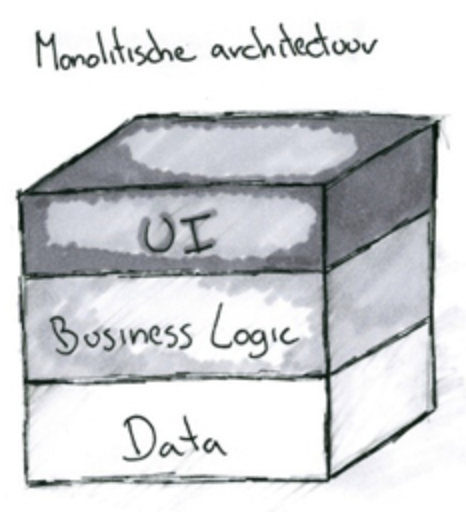
\includegraphics[width=80mm]{../monolith.png}
    \caption{Monolitische architectuur}
        
\end{figure}

Daarom is er een andere architectuur die een heel andere aanpak heeft, namelijk microservices. Dit bestaat uit verschillende kleinere componenten die indien nodig onafhankelijk van elkaar uitgevoerd kunnen worden. Bij deze aanpak is ook belangrijk dat je uw services klein houdt. Hierdoor kunnen je services gemakkelijk hergebruikt, begrepen en opnieuw gebuild worden. Iedere microservice heeft dus maar 1 verantwoordelijkheid.

Omdat microservices op verschillende machines moeten kunnen draaien, bijvoorbeeld op verschillende besturingssystemen, is het beter om ze in te pakken samen met hun dependencies in een container. \emph{Docker} is een voorbeeld van een technologie die deze containers aanbiedt. Door microservices in containers te plaatsen, zorg je ervoor dat de uitvoering van deze services onafhankelijk gebeurd met andere applicaties op dezelfde machine. Containers zijn dus onafhankelijk van een besturingssysteem, hierdoor kunnen microservices op verschillende locaties gedraaid worden. Een van de voordelen hiervan is dat ze door containers in de cloud kunnen geprogrammeerd worden.

De vier grootste voordelen van microservices zijn: 
\begin{itemize}
    \item Schaalbaarheid
    \item Beperken complexiteit
    \item Verkorten time-to-market
    \item Autonomie van ontwikkelteams.
\end{itemize}



 \autocite{Claudio2017} en \autocite{Velthoven2016}

\section{Kafka}

Wanneer je als bedrijf veel berichten binnen krijgt op een korte tijdsspanne, dan heb je natuurlijk een goed functionerende technologie nodig die al deze berichten kan verwerken. \emph{Kafka} is een voorbeeld van zo een technologie. Het is dus een berichtensysteem waarbij schaalbaarheid en redundantie een grote troef zijn. Bepaalde kernwoorden zijn belangrijk om de architectuur van \emph{Kafka} te begrijpen. Deze kernwoorden zijn: topics, producers, consumers en brokers.  

Topics zijn, zoals de naam al doet vermoeden, verschillende onderwerpen. Alle berichten zijn gegroepeerd in een van deze topics. Het formaat van een bericht kan verschillend zijn. Het type kan een gewone tekst zijn, kan van een Json-formaat zijn, of kan iets helemaal anders zijn. Het is mogelijk om zowel naar een specifieke topic een bericht te verzenden als te ontvangen. Dit brengt ons naadloos bij de volgende twee begrippen: producers en consumers. Als een producer kun je een bericht verzenden naar uw gewenste topic. Een consumer kan dan zelf bepalen van welke topic hij berichten wilt ontvangen. Het laatste woord dat nog moet verduidelijkt worden is een broker. \emph{Kafka} draait op een cluster. Iedere cluster bestaat uit één of meerdere nodes(servers). Zo een server noemen we een Kafka broker. Per Kafka cluster kunnen er verschillende producers en consumers zijn, zoals te zien is op figuur 2.2. 

\begin{figure}[h!]
    \centering
    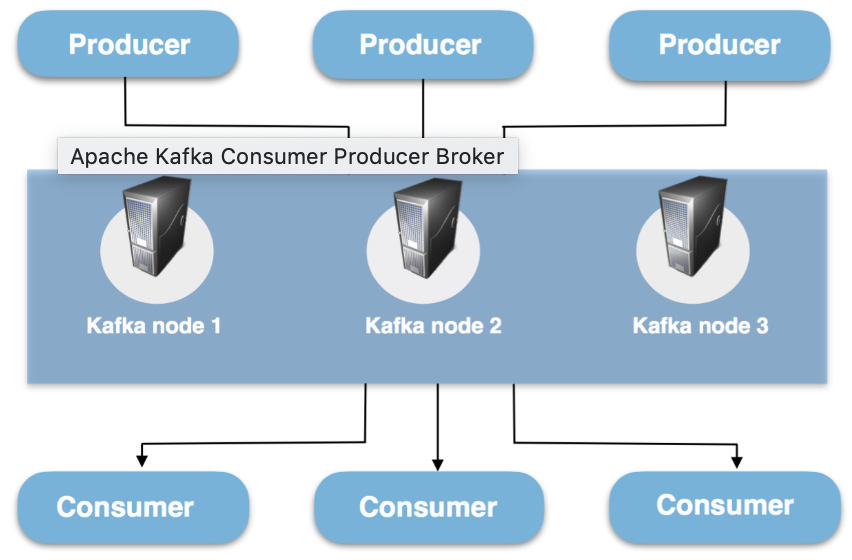
\includegraphics[width=80mm]{../kafkaCluster.png}
    \caption{Voorbeeld van een Kafka cluster}
    
\end{figure}

 Een topic kan je verdelen in verschillende partities. Dit wil zeggen dat je uw data kunt verdelen in ongeveer gelijke groepen (brokers). Iedere partitie kan dan staan voor een specifieke groep data binnen een topic zodat je niet alle berichten altijd moet overlopen. Dit principe van verschillende partities worden ook gebruikt bij traditionele databanken. Ook consumers kun je verdelen in verschillende partities, die samen één consumer-groep vormen. Door topics en consumers op deze manier op te delen, zorg je ervoor dat het mogelijk is dat meerdere consumers kunnen lezen van meerere partities in een topic. Dit heeft als positief gevolg dat je meer berichten kunt verwerken binnen een bepaalde tijd. 
 
 Ieder bericht binnen een partitie heeft een offset. Dit is een identifier, waardoor het mogelijk is om de berichten te ordenen. Normaal gezien als je als consumer je een subscriptie maakt op een topic, dan krijg je vanaf dit moment alle nieuwe berichten die binnen komen op de partitie waarop je een subscriptie hebt. Door een offset is het mogelijk om iets oudere berichten die op een partitie staan dan het moment dat je een subscriptie aangemaakt hebt, ook op te vragen. Op figuur 2.3 zie je een simpele voorstelling van een producer die berichten op een partitie van een topic plaatst. De cijfertjes stellen de offset voor van een bericht.
 \begin{figure}[h!]
     \centering
     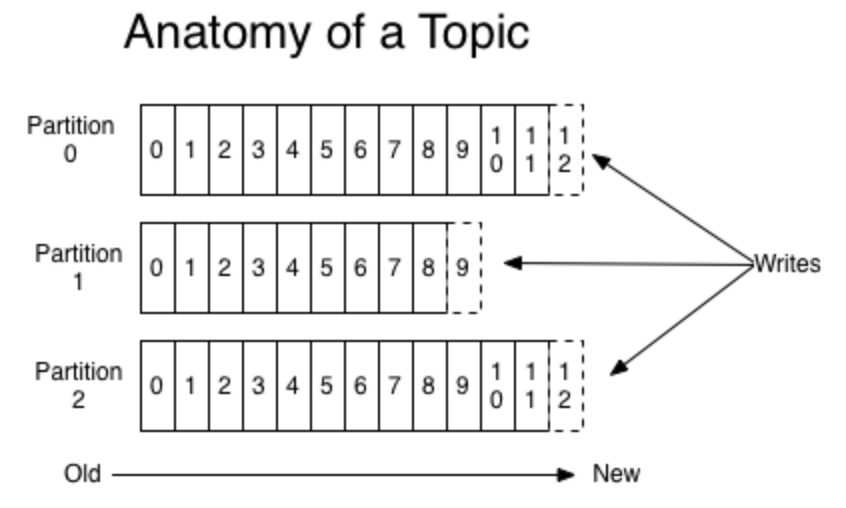
\includegraphics[width=80mm]{../kafkaOffset.png}
     \caption{Simpele voorstelling van de werking van een offset}
     
 \end{figure}

Het is al even vermeld, maar wat is nu eigenlijk een consumer-groep? Dit is een verzameling van verschillende consumers. Iedere consumer op zich leest van één specifieke partitie waardoor je het aantal berichten binnen één tijdseenheid kunt verhogen. Alle consumers binnen één groep lezen samen alle berichten die op een topic staan. Het opdelen van je topic in verschillende partities zorgt er dus niet voor dat je een deel van je data verliest. Mochten er meer consumers zijn dan dat er partities zijn, dan zitten er sommigen zonder werk. Omgekeerd, als er meer partities zijn dan consumers, dan krijgen consumers van verschillende partities berichten binnen.  Figuur 2.4 is een voorbeeld hoe een topic in verschillende servers kan opgedeeld worden en hoe consumers in consumer-groepen kunnen onderverdeeld worden. Je ziet dat de Kafka cluster in twee servers onderverdeelt is. Iedere server heeft twee partities. Er zijn 2 consumer-groepen, groep A bestaat uit twee consumers, groep B bestaat uit 4 consumers. Iedere partitie kan dus naar verschillende consumer-groepen berichten versturen, maar kan niet binnen dezelfde consumer-groep naar een andere consumer iets verzenden. 

 \begin{figure}[h!]
    \centering
    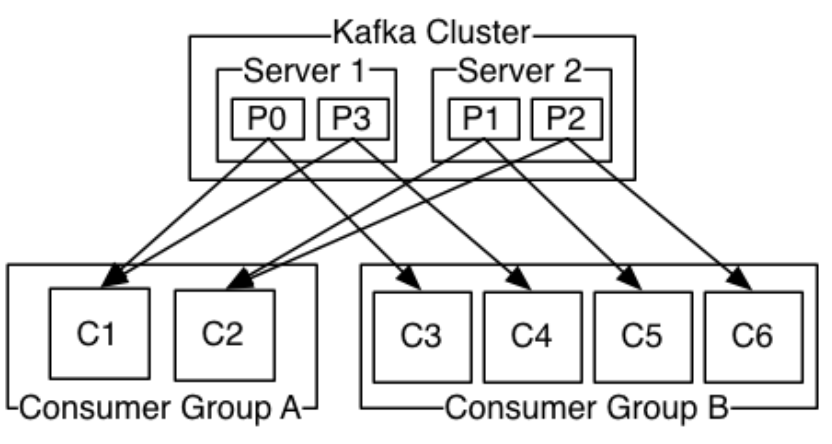
\includegraphics[width=80mm]{../kafkaConsumers.png}
    \caption{Wisselwerking tussen partities en consumer-groepen}
    
\end{figure}

\autocite{Sookocheff2015} en \autocite{Johansson2016}

\section{RabbitMq}

Een alternatief voor \emph{Kafka} is \emph{RabbitMq}. Dit is software waar men berichten kan plaatsen en ophalen op één of meerdere 'queues'. Ook hier heb je verschillende mogelijkheden van wat het formaat is van de berichten. Het kan zowel een gewone tekst zijn, als een Json-file. 

Wanneer een bericht van een queue wordt gelezen, dan wordt deze verwijderd van de queue. Het is dus niet mogelijk om later opnieuw hetzelfde bericht op te gaan vragen. De volledige queue kan ook een broker genoemd worden. Er zijn hier ook producers die data op de queue zetten, alsook consumers die een subscriptie kunnen maken op een queue. 




%%=============================================================================
%% Methodologie
%%=============================================================================

\chapter{Methodologie}
\label{ch:methodologie}
\lstset{
    tabsize = 4, %% Sets tab space width.
    showstringspaces = false, %% Prevents space marking in strings, string is defined as the text that is generally printed directly to the console.
    numbers = left, %% Displays line numbers on the left.
    commentstyle = \color{green}, %% Sets comment color.
    keywordstyle = \color{blue}, %% Sets  keyword color.
    stringstyle = \color{red}, %% Sets  string color.
    rulecolor = \color{black}, %% Sets frame color to avoid being affected by text color.
    basicstyle = \small \ttfamily , %% Sets listing font and size.
    breaklines = true, %% Enables line breaking.
    numberstyle = \tiny,
}

%%\begin{lstlisting}[language = Java , frame = trBL , firstnumber = last , escapeinside={(*@}{@*)}]
%%public class Factorial
%%{
%%public static void main(String[] args)
%%{   final int NUM_FACTS = 100;
%%for(int i = 0; i < NUM_FACTS; i++)
%%System.out.println( i + "! is " + factorial(i));
%%}
%%
%%public static int factorial(int n)
%%{   int result = 1;
%%for(int i = 2; i <= n; i++) (*@\label{for}@*)
%%result *= i;
%%return result;
%%}
%%}
%%\end{lstlisting}


%% TODO: Hoe ben je te werk gegaan? Verdeel je onderzoek in grote fasen, en
%% licht in elke fase toe welke stappen je gevolgd hebt. Verantwoord waarom je
%% op deze manier te werk gegaan bent. Je moet kunnen aantonen dat je de best
%% mogelijke manier toegepast hebt om een antwoord te vinden op de
%% onderzoeksvraag.

% TODO: uitleg wat we allemaal nodig hebben, producer uitleggen, consumer uitleggen, 3 verschillende groottes uitleggen.
Om te testen welke van de technologieën die in dit onderzoek aan bod komen nu eigenlijk het beste is, zou je met veel zaken rekening moeten houden. Wat het beste is hangt namelijk af van welke soort data je gebruikt. Ook de hoeveelheid transformaties die je data ondergaan voor dat het uitgelezen wordt of verzonden speelt een grote rol. Natuurlijk is het moeilijk om binnen de tijdspanne die er is voor dit onderzoek al deze factoren te gaan onderzoeken. Daarom zal dit onderzoek zich toespitsen op een bepaald scenario en daar conclusies uit trekken.  
\section{Producer project}
Het opzetten van een omgeving is per technologie verschillend. Elk heeft zijn eigen manier om data te verzenden en te ontvangen. Hieronder wordt eerst eens per technologie de implementatie getoond hoe we het project opgezet hebben. Daarna wordt er uitgelegd hoe we gaan testen welke nu de beste zal zijn. De reden waarom we specifiek deze technologieën gekozen hebben om te vergelijken kan opnieuw gelezen worden in de Stand van Zaken en de Inleiding.  

Natuurlijk moet er iets gelijkaardigs zijn om te kunnen vergelijken. Het data object dat we zullen verzenden en ontvangen bij zowel \emph{Kafka}, \emph{RabbitMq} en \emph{Google Pub/Sub} zal hetzelfde zijn. Op deze manier is het toekomstige resultaat niet afhankelijk van het type data. Dit onderzoek zal zich dus toespitsen op data met het type Json. Deze klasse (Data.class) hergebruiken we in elke technologie. Deze klasse is het type van het bericht dat we verzenden.
\begin{lstlisting}[language = Java , frame = trBL , firstnumber = last , escapeinside={(*@}{@*)}]
@Getter
@AllArgsConstructor
@NoArgsConstructor
@ToString
public class Data {
    private int id;
    private String name;
    private String description;
    private Date sendedDate;
}
     \end{lstlisting}
     
Deze klasse bevat vier attributen. Dit is om een Json object na te bootsen. Het is vanzelfsprekend dat deze klasse niet zo maar automatisch kan omgezet worden naar een Json. De manier waarop dit gedaan wordt is opnieuw per technologie verschillend. De uitleg zal gegeven worden in de subsectie van de technologie zelf hoe het omzetten gebeurd. De attributen die hier gebruikt worden zijn: een id van het type int, dit is om elk data object van elkaar te kunnen onderscheiden tijdens het verzenden. Als tweede zie je naam van het type String. Dit heeft als bedoeling opnieuw om verschillende objecten van elkaar te kunnen onderscheiden en om een realistische attribuut te geven aan het Data-object. Deze reden is hetzelfde voor het attribuut description van het type String. Als laatste hebben we de sendedDate van het type Date. Deze zal de datum en het tijdstip doorsturen van het moment wanneer het object verzonden is. Dit zal later nog eens aangehaald worden wanneer we deze objecten genereren. 

Als u boven de klasse kijkt dan ziet u nog vier annotaties staan. Deze kunnen we gebruiken door de library van lombok. Dit werd mogelijk gemaakt door deze dependency toe te voegen aan onze pom.xml want het gebruikte project voor dit onderzoek maakt gebruik van Maven om libraries toe te voegen.

\begin{lstlisting}[language = xml , frame = trBL , firstnumber = 1 , escapeinside={(*@}{@*)}]
<dependency>
<groupId>org.projectlombok</groupId>
<artifactId>lombok</artifactId>
<optional>true</optional>
</dependency>
\end{lstlisting}

Deze geeft op voorhand al enkele handige implementaties. De gebruikte annotaties zullen we uitleggen, want natuurlijk bestaan er meer dan enkel deze die dit onderzoek gebruikt. Voor de andere mogelijkheden verwijs ik u graag door naar de site van Project Lombok waar u alle mogelijkheden op een rijtje ziet: https://projectlombok.org/features/all. 

De eerste annotatie is @Getter, deze zorgt ervoor zoals de naam al doet vermoeden, dat er voor ieder attribuut een getter aanwezig is. Op deze manier staat uw code niet overvol met getters van al uw attributen. In deze klasse zijn er niet zo veel attributen dus zou het aantal getter nog meevallen. Maar u kan zich wel inbeelden dat in een groter project in een klasse met veel attributen en andere methodes dat dit een handige annotatie is. Je ziet dus niet dat de getters aanwezig zijn maar die zijn er wel effectief. Laten we de tweede en de derde samen bekijken: @AllArgsConstructor en @NoArgsConstructor. Deze zorgen ervoor dat er een constructor gegenereerd wordt met respectievelijk al de attributen en zonder de attributen. Deze zijn vaak voorkomende constructors en zijn handig om ook hiervoor een annotatie te hebben. De laatste  is de @ToString. Deze werd gebruikt tijdens de opmaak van het project. Dit vormt het object om in een String. Dit was handig om lokaal te testen. Het data object werd dan uitgeprint tijdens het verzenden om te controleren als het object wel de juiste waardes bevatte.
\subsection{Kafka}
In figuur 3.1 ziet u welke configuratie de topic heeft. Er wordt gebruik gemaakt van zes partities en de data wordt vier weken bijgehouden. Met andere woorden: als de data op de topic komt, en deze niet binnen de vier weken door een consumer, dan wordt de data verwijderd en kan deze data niet meer opnieuw uitgelezen worden.
\begin{figure}[h!]
    \centering
    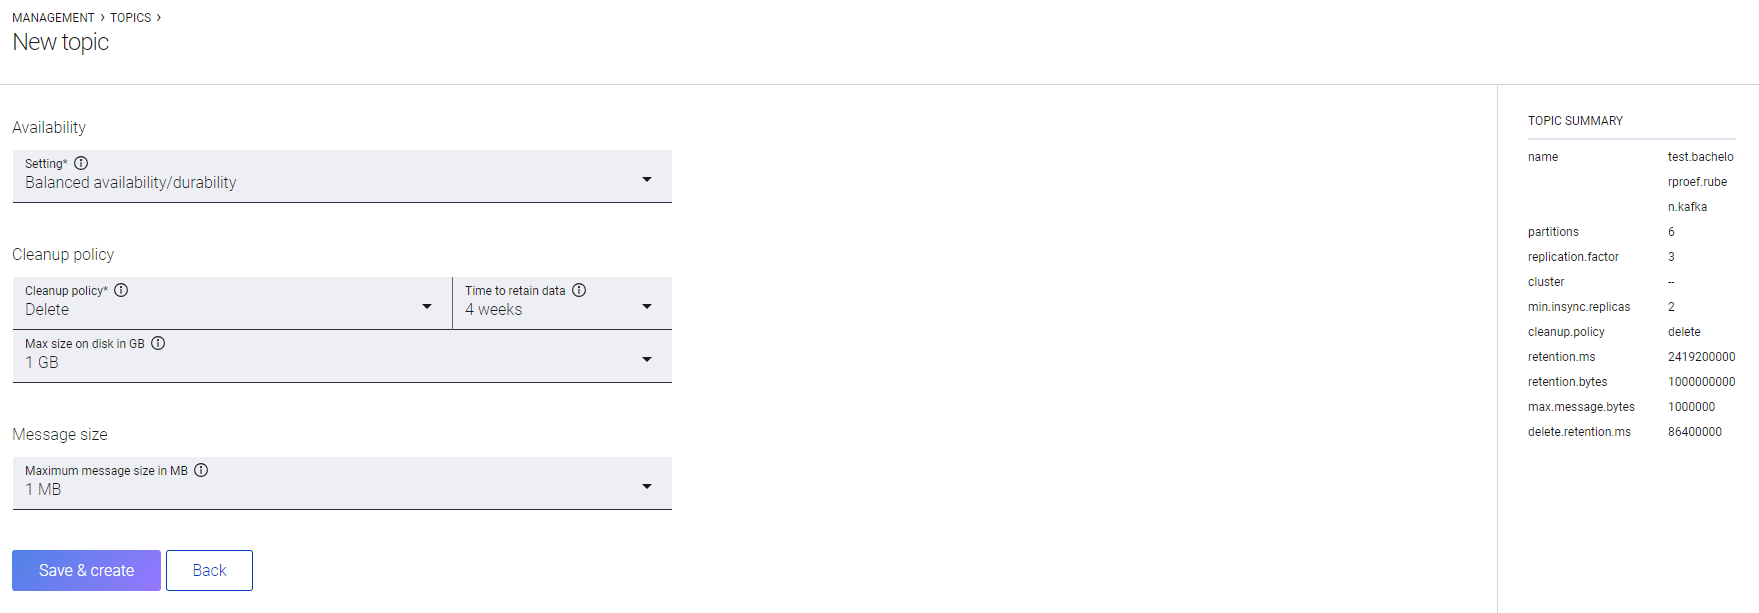
\includegraphics[width=140mm]{../kafkaConfig.png}
    \caption{Configuratie van de topic}
    
\end{figure}
\subsubsection{KafkaConfig}
Zo ziet de implementatie van de KafkaConfig.class eruit.

    \begin{lstlisting}[language = Java , frame = trBL , firstnumber = 1 , escapeinside={(*@}{@*)}]
    @Configuration
    public class KafkaConfig {
        
        @Bean
        @Primary
        public KafkaProperties kafkaProperties(
        @Value("${kafka_key}") final String kafkaKey,
        @Value("${kafka_secret}") final String kafkaSecret
        
        ) {
            KafkaProperties kafkaProperties = new KafkaProperties();
            
            KafkaProperties.Producer producer = kafkaProperties.getProducer();
            
            producer.getProperties().put(ProducerConfig.KEY_SERIALIZER_CLASS_CONFIG, "org.apache.kafka.common.serialization.StringSerializer");
            producer.getProperties().put(ProducerConfig.VALUE_SERIALIZER_CLASS_CONFIG, "org.springframework.kafka.support.serializer.JsonSerializer");
            
            producer.getProperties().put(ProducerConfig.BOOTSTRAP_SERVERS_CONFIG, "pkc-412nj.europe-west1.gcp.confluent.cloud:9092");
            producer.getProperties().put(ProducerConfig.RETRIES_CONFIG, "0");
            producer.getProperties().put(ProducerConfig.ACKS_CONFIG, "all");
            producer.getProperties().put(ProducerConfig.RETRY_BACKOFF_MS_CONFIG, "1000");
            producer.getProperties().put(ProducerConfig.REQUEST_TIMEOUT_MS_CONFIG, "30000");
            producer.getProperties().put(ProducerConfig.LINGER_MS_CONFIG, "200");
            kafkaProperties.getProperties().put(SslConfigs.SSL_ENDPOINT_IDENTIFICATION_ALGORITHM_CONFIG, "https");
            kafkaProperties.getProperties().put(SaslConfigs.SASL_MECHANISM, "PLAIN");
            kafkaProperties.getProperties().put("request.timeout.ms", "20000");
            kafkaProperties.getProperties().put("retry.backoff.ms", "500");
            kafkaProperties.getProperties().put(SaslConfigs.SASL_JAAS_CONFIG, "org.apache.kafka.common.security.plain.PlainLoginModule required username=\""
            + kafkaKey + "\" password=\"" + kafkaSecret + "\";");
            kafkaProperties.getProperties().put("security.protocol", "SASL_SSL");
            
            kafkaProperties.getProperties().put(JsonSerializer.ADD_TYPE_INFO_HEADERS, "false");
            
            return kafkaProperties;
        }
            \end{lstlisting}
            
     In deze klasse ziet u dat het instellen van de nodige properties in de kafkaProperties methode van deze klasse gebeurd. Deze zouden ook in de application.yml file kunnen ingesteld worden. In dit project van het onderzoek hebben we besloten om dit in een config klasse te doen. Tijdens het opzetten van het project kon de applicatie de properties niet uitlezen vanuit de application.yml file. Om geen tijd te verliezen hebben we besloten om deze properties in een config klasse in te stellen. Dit verandert niets van functionaliteit of aan resultaten van dit onderzoek. Maar als onderzoeker was het mogelijk om sneller aan de slag te gaan met het belangrijkere werk.
     
     Boven de klasse ziet u de annotatie @Configuration. Dit is een annotatie van het Spring framework. Deze zorgt ervoor dat je aangeeft dat deze klasse een configuratie instelt. In de klasse ziet u boven de methode kafkaProperties twee andere annotaties staan. @Bean zorgt ervoor dat er een bean aangemaakt wordt voor deze methode. Dit zorgt ervoor dat door het Spring framework voor deze methode eerder een instantie aangemaakt wordt en daardoor de applicatie bij het opstarten deze properties kan instellen. Daaronder zie je een andere annotatie die hiermee te maken heeft: @Primary. Deze zorgt ervoor als het Spring framework meerdere beans heeft van KafkaProperties, dat hij deze voorneemt op al de andere. Op deze manier zijn we zeker dat deze properties gebruikt worden en niet andere indien er meerdere beans zouden zijn.
     
     U ziet dat er tamelijk wat properties geconfigureerd zijn. Er zullen slechts enkele properties besproken worden, uiteraard zijn dit de belangrijkste voor dit onderzoek. In dit hoofdstuk werd al eens vermeld dat het object van de klasse Data niet zomaar omgezet wordt naar een Json. Hiervoor is er een serializer nodig die dit doet. Op lijn 16 van de KafkaConfig klasse is er te zien dat de gekozen serializer ingesteld wordt. In dit geval wordt de JsonSerializer gebruikt uit de package springframework.kafka.support.serializer. Dit is dus een specifieke JsonSerializer voor Kafka. De key wordt dan weer geserializeerd naar een String door de StringSerializer uit de package org.apache.kafka.common.serialization, dit is te zien op de regel er boven. Wat als het niet lukt voor de producer om de data te verzenden? In ons geval mag hij dit niet opnieuw proberen. Op deze manier kunnen we ook te weten komen hoeveel data er mislukt is om te verzenden. Dit zie je op lijn 19. Indien je meer zekerheid wilt dat je een data object zeker verzonden wordt, dan kan je deze property in plaats van 0 op bijvoorbeeld 3 zetten. Je mag zeker ook niet vergeten om de username en password mee te geven van waar je Kafka topic zich bevindt. Op lijn 28 en 29 zie je dat dit meegegeven wordt. De username en wachtwoord worden niet in plaintext in de code geplaatst. Het is niet de bedoeling dat iedereen weet wat het wachtwoord en username is. Deze worden ingesteld in uw application.yml en worden meegegeven via de parameters van de methode door het spring framework. Door de annotatie @Value en de naam van de key van uw waarden in de application.yml, weet spring perfect waar hij het wachtwoord en username moet gaan halen.
     
    \subsubsection{KafkaPublisher}
    De KafkaPublisher.class is de effectieve producer van Data objecten. Veel moet er niet ingesteld worden om deze producer te doen laten werken. Wat je zeker moet hebben is een KafkaTemplate en de naam van de topic waarnaar je verzend. Laat ons even deze klasse stap voor stap bekijken.
    
    Boven de klasse staat de annotatie @Component. Dit is opnieuw een annotatie van het spring framework. Deze zorgt ervoor dat je via constructor- of setterinjectie in andere klasses telkens dezelfde instantie van de klasse KafkaPublisher kunt gebruiken. Op die manier moet je niet telkens een nieuwe instantie maken van de klasse. Er zijn twee attributen: de kafkaTemplate van het type KafkaTemplate en een String topicName; De KafkaTemplate is een template die je gebruikt om je message naar een Kafka topic te verzenden.
    
    In de constructor worden kafkaTemplate en topicName meegegeven als parameters. Spring Boot zorgt ervoor dat de kafkaTemplate automatisch gecreëerd wordt. De topicName willen we niet zo maar in onze code schrijven, dus injecteren we die vanuit de application.yml. Hiervoor wordt opnieuw @Value gebruikt, maar dit principe werd al eens uitgelegd.
    
    Als laatste bevat deze klasse ook nog de publish methode. Deze verzend een message effectief naar de topic. In onze implementatie krijgt deze methode een lijst van Data objecten mee. In dit onderzoek is het niet van toepassing om één enkel Data object te verzenden, dus om praktische redenen wordt er een lijst meegegeven. In deze methode wordt deze lijst overlopen en telkens worden dezelfde operaties uitgevoerd. Er wordt een object aangemaakt van de klasse Message, zoals de naam al doet vermoeden wordt dit onze message. In de payload van deze message stoppen we ons Data object. In de header geven we twee zaken mee. Als message key geven we het id mee, omdat in deze implementatie het id toch telkens uniek zal zijn. Als tweede moeten we nog de naam van onze topic meegeven zodat de kafkaTemplate weet naar waar hij moet versturen. Het enigste dat deze methode dan nog moet doen is de kafkaTemplate gebruiken om de message te verzenden. Het omzetten van de message in een json formaat wordt automatisch gedaan omdat we in de properties een serializer opgegeven hebben. Ook de message key wordt voor dezelfde reden automatisch geserializeerd. 
 
        \begin{lstlisting}[language = Java , frame = trBL , firstnumber = 1 , escapeinside={(*@}{@*)}]
    @Component
    public class KafkaPublisher {
        
        private KafkaTemplate kafkaTemplate;
        private String topicName;
        
        public KafkaPublisher(KafkaTemplate kafkaTemplate,
        @Value("${kafka.topic.name}") String topicName) {
            this.kafkaTemplate = kafkaTemplate;
            this.topicName = topicName;
        }
        
        public void publish(List<Data> dataList) {
            for (Data data : dataList) {
                Message<Data> message = MessageBuilder.withPayload(data)
                .setHeader(KafkaHeaders.MESSAGE_KEY, String.valueOf(data.getId()))
                .setHeader(KafkaHeaders.TOPIC, topicName)
                .build();
                
                kafkaTemplate.send(message);
            }
        }
    }
     \end{lstlisting}
\subsection{RabbitMq}
\subsubsection{RabbitMqConfig}
In dit onderzoek zijn alle configuraties van RabbitMq gedaan in application.yml. 
        \begin{lstlisting}[language = xml , frame = trBL , firstnumber = 1 , escapeinside={(*@}{@*)}]
spring:
    rabbitmq:
        host: "hostadress"
        port: 16379
        username: ${rabbitmq_username}
        password: ${rabbitmq_password}
        virtual-host: "rabbitmq"
        ssl:
            enabled: true
            algorithm: "TLSv1.2"
        listener:
         simple:
            default-requeue-rejected: false
        direct:
            default-requeue-rejected: false
     \end{lstlisting}
     
     Veel configuraties zijn er niet. De belangrijkste zijn host, port, username en password. De host is het adres waar uw RabbitMq exchange op draait met de juiste poort die opgegeven wordt in port. In het project is de String ''hostadress'' vervangen door de effectieve host. Om privacy redenen is hier dit adres gewijzigd. Username en password worden ook nog bijgehouden in een variabele maar deze staan natuurlijk niet op het codevoorbeeld. Hiernaast wordt ook nog de naam van de exchange bijgehouden die we later in de implementatie nodig zullen hebben. Uiteraard zit deze property ook niet in het codevoorbeeld.
     
 \subsubsection{RabbitMqPublisher}
 Over het algemeen gezien kun je deze klasse goed vergelijken met de KafkaPublisher klasse. Het grootste verschil zit men in de publish methode. De annotatie @Component boven de klasse heeft hetzelfde doel als bij de KafkaPublisher. Er is hier één attribuut meer en dat is de ObjectMapper. Deze wordt gebruikt om later in de publish methode onze data om te zetten naar een String. Uiteraard is de KafkaTemplate hier vervangen door een RabbitTemplate. Deze hebben dezelfde functionaliteit maar bij een verschillende technologie. Het is dus ook een template die je gebruikt om de data te verzenden naar de exchange. Hier heb je niet de naam van de topic nodig zoals bij de KafkaPublisher maar de naam van de exchange.
 
 In de constructor wordt de rabbitTemplate en de objectMapper opnieuw automatisch gecreëerd door Spring Boot. De naam van de exchange wordt weer via de application.yml file geïnjecteerd. In de publish methode overlopen we weer een lijst van objecten van Data. Bij iedere elementje uit de lijst voeren we dezelfde operaties uit. We gebruiken de objectMapper om ons object om te zetten naar een String. Het resultaat van deze String is in een Json formaat. Dit kunnen we ook verifiëren en daarom is als laatste lijn in de for-lus een print-statement toegevoegd. Deze String wordt uitgeprint en we kunnen mooi zien dat deze String een Json formaat heeft. Verder gebruiken we de rabbitTemplate om ons bericht te verzenden naar de exchange die we meegeven samen met ons bericht.
   \begin{lstlisting}[language = java , frame = trBL , firstnumber = 1 , escapeinside={(*@}{@*)}]
 @Component
 public class RabbitMqPublisher {
     private RabbitTemplate rabbitTemplate;
     private ObjectMapper objectMapper;
     private String exchangeName;
     
     public RabbitMqPublisher(final RabbitTemplate rabbitTemplate,
     final ObjectMapper objectMapper,
     @Value("${rabbitmq.topic.exchange.name}") final String exchangeName) {
         this.rabbitTemplate = rabbitTemplate;
         this.objectMapper = objectMapper;
         this.exchangeName = exchangeName;
     }
     
     public void publish(final List<Data> dataList) {
         try {
             for (Data data : dataList) {
                 String stringData = objectMapper.writeValueAsString(data);
                 
                 rabbitTemplate.convertAndSend(exchangeName, "", stringData);
                 System.out.println("sending messeage RMQ: " + stringData);
             }
             
         } catch (JsonProcessingException e) {
             e.printStackTrace();
         }
     }
 }
     \end{lstlisting}
\subsection{Google Pub/Sub}
Op figuur 3.2 kunt u zien hoe de configuratie van de topic is voor de gebruikte subscription in dit onderzoek. We zien dat bij het lezen van een message die op de Pub/Sub staat, dat er een tijdlimiet staat van 60 seconden. Dit wil zeggen dat indien de message binnen de 60 seconden niet gelezen kan worden wanneer de subscriber messages aan het lezen is, dat de actie NACK uitgevoerd wordt op deze message. Dit wil zeggen dat de message nog altijd niet verwijderd is van de topic en dat deze nog altijd gelezen kan worden door de subscriber. Bij Google Pub/Sub kun je deze tijdslimiet instellen tussen 60 en 600 seconden. Onder de ''Acknowledgement''' Deadline ziet u ''Message retention duration'' staan. Dit is hoe lang een message op de topic blijft staan. In dit geval staat deze waarde op het maximum: op zeven dagen. Met andere woorden: indien een message binnen de zeven dagen niet gelezen wordt, dan zal deze verwijderd worden en is het niet meer mogelijk om deze message terug te vinden.
\begin{figure}[h!]
    \centering
    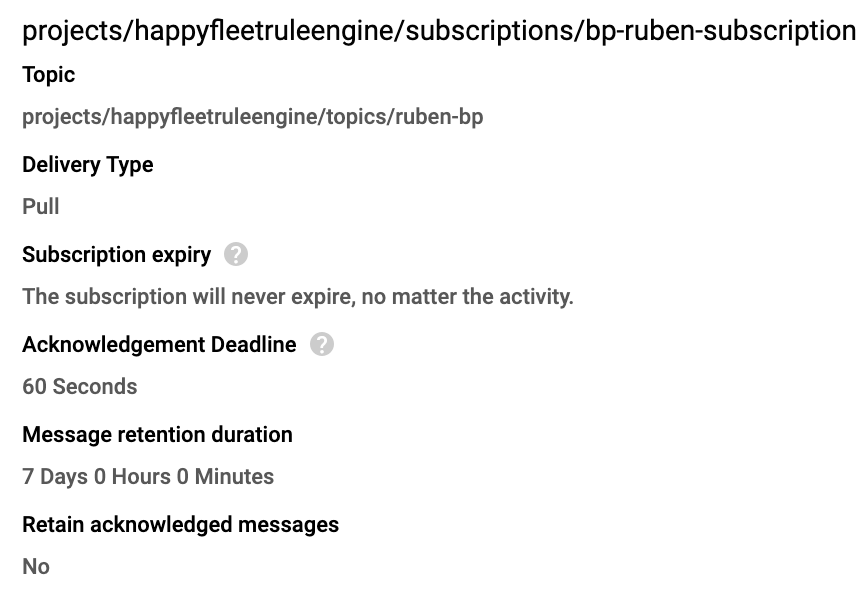
\includegraphics[width=140mm]{../gpsConfig.png}
    \caption{Configuratie van de topic voor de gebruikte subscription}
    
\end{figure}
\subsubsection{GooglePubSubConfig}
Zo ziet de GooglePubSubConfig.class eruit. Er worden twee kanalen aangemaakt van het type MessageChannel. Deze kanalen worden gebruikt om een bericht van een topic te lezen of verzenden.
        \begin{lstlisting}[language = Java , frame = trBL , firstnumber = last , escapeinside={(*@}{@*)}]
@Configuration
public class GooglePubSubConfig {
    @Bean("bachelorproef-channel-input")
    public MessageChannel createDeviceEventChannelInput() {
        return new DirectChannel();
    }
    
    @Bean("bachelorproef-channel-output")
    public MessageChannel createDeviceEventChannelOutput() {
        return new DirectChannel();
    }
    
    @Bean
    public PubSubInboundChannelAdapter createDeviceChannelAdapter(
    PubSubOperations pubSubTemplate,
    @Value("${pubsub.subscription}") String subsciptionName,
    @Qualifier("bachelorproef-channel-input") MessageChannel inputChannel,
    @Value("${pubsub.autostartup}") Boolean autoStart) {
        
        final PubSubInboundChannelAdapter adapter = new PubSubInboundChannelAdapter(pubSubTemplate, subsciptionName);
        adapter.setOutputChannel(inputChannel);
        adapter.setAckMode(AckMode.AUTO);
        adapter.setPayloadType(Event.class);
        adapter.setAutoStartup(autoStart);
        return adapter;
    }
    
    @Bean
    @ServiceActivator(inputChannel = "bachelorproef-channel-output")
    public MessageHandler messageSender(
    PubSubOperations pubsubTemplate,
    @Value("${pubsub.topic}") String topicName
    ) {
        return new PubSubMessageHandler(pubsubTemplate, topicName);
    }
    
    @Bean
    public JacksonPubSubMessageConverter createJacksonMessageConverter(final ObjectMapper objectMapper) {
        return new JacksonPubSubMessageConverter(objectMapper);
    }
    
}
     \end{lstlisting}
\subsubsection{GooglePubSubPublisher}
Deze klasse heeft maar één methode, namelijk publishData. Deze methode verstuurd het Data-object naar de topic via het kanaal \emph{bachelorproef-channel-output}. Er hoeft geen implementatie te zijn van deze methode, het spring-framework regelt al het andere werk in jouw plaats.
        \begin{lstlisting}[language = Java , frame = trBL , firstnumber = last , escapeinside={(*@}{@*)}]
@MessagingGateway(defaultRequestChannel = "bachelorproef-channel-output")
@Component
public interface GooglePubSubPublisher {
    void publishData(Data data);
    
}
     \end{lstlisting}
     
\section{Consumer project}
\section{Onderzoek}



% Voeg hier je eigen hoofdstukken toe die de ``corpus'' van je bachelorproef
% vormen. De structuur en titels hangen af van je eigen onderzoek. Je kan bv.
% elke fase in je onderzoek in een apart hoofdstuk bespreken.

%\input{...}
%\input{...}
%...

%%=============================================================================
%% Conclusie
%%=============================================================================

\chapter{Conclusie}
\label{ch:conclusie}

%% TODO: Trek een duidelijke conclusie, in de vorm van een antwoord op de
%% onderzoeksvra(a)g(en). Wat was jouw bijdrage aan het onderzoeksdomein en
%% hoe biedt dit meerwaarde aan het vakgebied/doelgroep? Reflecteer kritisch
%% over het resultaat. Had je deze uitkomst verwacht? Zijn er zaken die nog
%% niet duidelijk zijn? Heeft het onderzoek geleid tot nieuwe vragen die
%% uitnodigen tot verder onderzoek?

\section{Snelheid}
\subsection{10 000 objecten}
Het eerste wat we gaan analyseren en een conclusie uit trekken is het verzenden van 10 000 objecten. Eerst kijken we naar de waardes apart per technologie, daarna gaan we alle technologieën gaan vergelijken met elkaar.
\subsubsection{Google Pub/Sub}
De resultaten van de snelheden bij 10 000 objecten van Google Pub/Sub zien er als volgt uit:
\begin{table}[h!]
    \centering
    \label{q1}
    \begin{tabular}{| 1 | c |}
        \hline
        & Tijd (ms)\\ \hline
        min. & 1366  \\
        gem. & 11665.7694 \\
        max. & 19365\\
        \# ontvangen. & 10 000\\ \hline
    \end{tabular}
    \caption{Verschil tussen ontvangen en verzenden (in ms) - Google Pub/Sub}
\end{table}

We zien dus dat het kleinste verschil iets meer dan één seconde is, en het grootste verschil bijna 20 seconden. Het gemiddeld aantal seconden ligt rond de 11,5 seconden.

\subsubsection{Kafka}
De resultaten van de snelheden bij 10 000 objecten van Kafka zien er als volgt uit:
\begin{table}[h!]
    \centering
    \label{q1}
    \begin{tabular}{| 1 | c |}
        \hline
        & Tijd (ms)\\ \hline
        min. & 1008  \\
        gem. & 20339.5169 \\
        max. & 38537\\
        \# ontvangen. & 10 000\\ \hline
    \end{tabular}
    \caption{Verschil tussen ontvangen en verzenden (in ms) - Kafka}
\end{table}

We zien dus dat het kleinste verschil nog dichter bij de één seconde ligt dan bij Google Pub/Sub. Het grootste verschil is bijna 40 seconden. Het gemiddeld aantal seconden ligt rond de 20 seconden.

\subsubsection{RabbitMq}
De resultaten van de snelheden bij 10 000 objecten van RabbitMq zien er als volgt uit:
\begin{table}[h!]
    \centering
    \label{q1}
    \begin{tabular}{| 1 | c |}
        \hline
        & Tijd (ms)\\ \hline
        min. & 598  \\
        gem. & 21780.9111 \\
        max. & 41805\\
        \# ontvangen. & 10 000\\ \hline
    \end{tabular}
    \caption{Verschil tussen ontvangen en verzenden (in ms) - RabbitMq}
\end{table}

Het kleinste tijdverschil is iets meer dan een halve seconde. Het grootste verschil is meer dan 40 seconden. Het gemiddeld aantal seconden is bijna 42 seconden.
\subsubsection{Vergelijking}
Om een goede vergelijking te kunnen maken tussen de drie technologieën zetten we de resultaten bij 10 000 objecten van de verschillende technologieën even naast elkaar met behulp van drie boxplots die te zien is op figuur 5.1.

 \begin{figure}[h!]
    \centering
    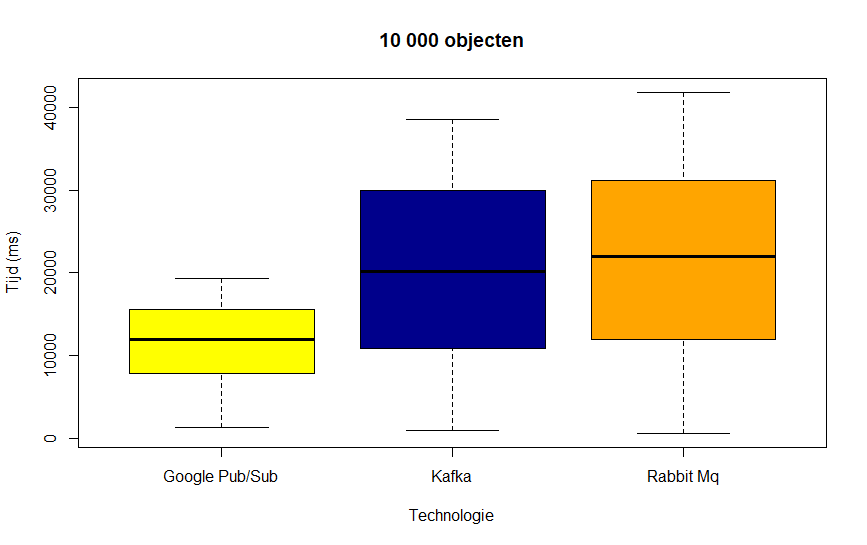
\includegraphics[width=100mm]{../10000Boxplot.png}
    \caption{Vergelijking bij 10 000 objecten}
    
\end{figure}

Bij zowel Google Pub/Sub, Kafka en RabbitMq zijn alle 10 000 objecten die verzonden zijn geweest, ook aangekomen. Dit wil zeggen dat bij 10 000 objecten geen enkel object mislukt is om te ontvangen. We kunnen bij deze hoeveelheid dus een duidelijke conclusie trekken als we kijken naar de snelheid tussen ontvangen en verzenden. 

Eerst bekijken we de minimum waarden. Daarin is te zien dat RabbitMq de kortste tijd heeft van de drie minimum waarden. Dit is dubbel zo snel als we vergelijken met Kafka, die de tweede kortste tijd heeft. RabbitMq slaagt er in om in ongeveer een halve seconde een object te verzenden en te ontvangen. Kafka doet dit slechts in één seconde. Google Pub/Sub is de slechtste leerling van de klas op het gebied van minimum tijd en doet er ongeveer 1,3 seconden over.

Laat ons nu kijken naar de maximum tijd. Hier doet Google Pub/Sub het veruit beter of de twee andere technologieën. Het doet er nooit langer dan 20 seconden over om een bericht te versturen en weer te lezen. Hier doen Kafka en RabbitMq het veel slechter. Zij doen er maximum 3,8 en 4,1 seconde over, en dit is veel meer of bij Google Pub/Sub.

Het resultaat van de maxima weerspiegelt zich ook in de gemiddeldes. Gemiddeld doet Google Pub/Sub er 11 seconden over. Het gemiddelde van Kafka en RabbitMq ligt dan weer wat hoger met 20 en 21 seconden.

Conclusie bij 10 000 objecten: Alhoewel de minimum tijd bij Google Pub/Sub hoger ligt of bij Kafka en RabbitMq, slaagt Google Pub/Sub er toch in om behoorlijk wat sneller al de data te verwerken. 


\subsection{100 000 objecten}
Het lijkt ons ook interessant om eens te bekijken wat te resultaten zijn indien we het aantal objecten wat gaan verhogen. We nemen tien keer zo veel objecten en kijken wat we hiermee kunnen uit concluderen.
\subsubsection{Google Pub/Sub}
De resultaten van de snelheden bij 100 000 objecten van Google Pub/Sub zien er als volgt uit:
\begin{table}[h!]
    \centering
    \label{q1}
    \begin{tabular}{| 1 | c |}
        \hline
        & Tijd (ms)\\ \hline
        min. &  1753\\
        gem. & 88603.80396 \\
        max. & 169580\\
        \# ontvangen. & 100 000\\ \hline
    \end{tabular}
    \caption{Verschil tussen ontvangen en verzenden (in ms) - Google Pub/Sub}
\end{table}

We zien dus dat het kleinste verschil iets minder is dan twee seconden, en het grootste verschil bijna 170 seconden, wat bijna drie minuten is. Het gemiddeld aantal seconden ligt rond de 88 seconden, wat bijna 1,5 minuten is.

\subsubsection{Kafka}
De resultaten van de snelheden bij 100 000 objecten van Kafka zien er als volgt uit:
\begin{table}[h!]
    \centering
    \label{q1}
    \begin{tabular}{| 1 | c |}
        \hline
        & Tijd (ms)\\ \hline
        min. & 1055  \\
        gem. & 175526.39283 \\
        max. & 346431\\
        \# ontvangen. & 100 000\\ \hline
    \end{tabular}
    \caption{Verschil tussen ontvangen en verzenden (in ms) - Kafka}
\end{table}

Het kleinste verschil blijft nog steeds dicht bij de één seconde liggen, alhoewel het verschil toch lichtjes gestegen is. Het grootste verschil ligt rond de 346 seconden, wat bijna zes minuten is. Het gemiddeld aantal seconden ligt rond de 175 seconden, omgerekend is dit bijna drie minuten.

\subsubsection{RabbitMq}
De resultaten van de snelheden bij 100 000 objecten van RabbitMq zien er als volgt uit:
\begin{table}[h!]
    \centering
    \label{q1}
    \begin{tabular}{| 1 | c |}
        \hline
        & Tijd (ms)\\ \hline
        min. & 458  \\
        gem. & 114365.12135045651 \\
        max. & 224467\\
        \# ontvangen. & 59 802\\ \hline
    \end{tabular}
    \caption{Verschil tussen ontvangen en verzenden (in ms) - RabbitMq}
\end{table}

Wat meteen opvalt, is dat bij deze hoeveelheid RabbitMq er niet in geslaagd is om tijdens dezelfde run alle 100 000 objecten binnen te halen. Natuurlijk haalt hij deze wel nog binnen indien de applicatie opnieuw opgestart wordt, maar het is toch opvallend dat maar iets meer of de helft meteen ontvangen wordt.

De minimum tijd is nog gedaald in vergelijking met 10 000 objecten. Hij heeft nu slechts minder dan een halve seconde nodig om te verzenden en te ontvangen. Het gemiddelde ligt rond de 114 seconden en het maximum iets meer dan 224 seconden. Natuurlijk zijn het gemiddelde en maximum minder belangrijk om te vergelijken aangezien niet alle 100 000 objecten zijn ontvangen.
\subsubsection{Vergelijking}
Ook bij deze hoeveelheid aan objecten zetten we de drie technologieën eens naast elkaar. Deze boxplots zijn te zien op figuur 5.2

\begin{figure}[h!]
    \centering
    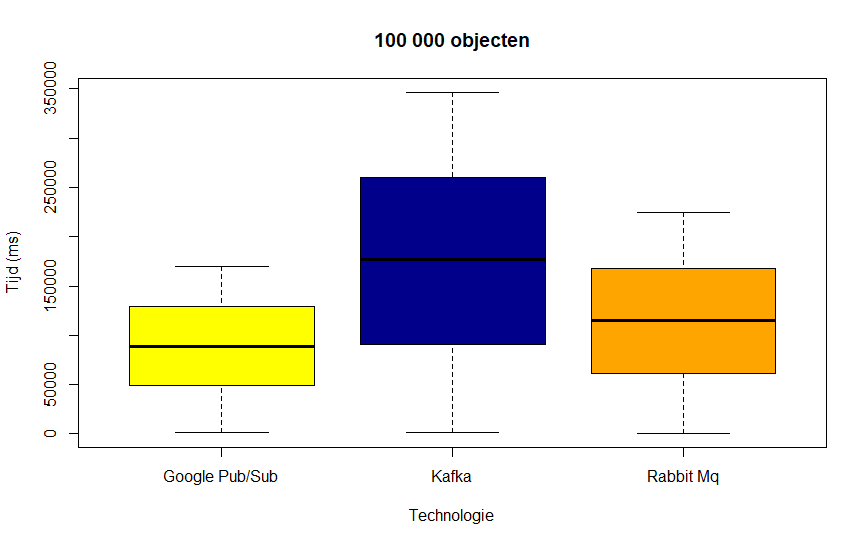
\includegraphics[width=100mm]{../100000Boxplot.png}
    \caption{Vergelijking bij 100 000 objecten}
    
\end{figure}

Hierbij is het minder relevant om RabbitMq helemaal te gaan vergelijken met de twee andere technologieën aangezien maar iets meer dan de helft van de objecten ook ontvangen zijn geweest.

Eerst gaan we de minimum waarden bekijken, hier kunnen we ook nog vergelijken met RabbitMq. Daarin is te zien dat RabbitMq de kortste tijd heeft van de drie minimum waarden. Deze waarde is zelf nog minder dan bij de vorige vergelijking van 10 000 objecten. Kafka blijft redelijk stabiel van de kortste tijd en schommelt nog steeds rond de seconde. Bij Google Pub/Sub zien we toch een stijging en deze waarde is nu 1,7 seconden geworden.

Laat ons nu kijken naar de maximum tijd. Hier doet opnieuw Google Pub/Sub het veruit beter of de twee andere technologieën. We zouden kunnen zeggen dat de waarde bij RabbitMq ook nog goed meevalt, maar dit zou een vertekend beeld geven omdat niet alle objecten ontvangen zijn geweest. Dus het heeft enkel zin om voor de maximum waarde Google Pub/Sub te gaan vergelijken met Kafka. Bij Kafka ligt de maximum waarde veel hoger. Het heeft er maximum ongeveer 346 seconden voor nodig, wat bijna dubbel zo veel is dan bij Google Pub/Sub.

Het resultaat van de maxima weerspiegelt zich ook opnieuw in de gemiddeldes. Ook hier houden we geen rekening met RabbitMq want niet alle objecten zijn ontvangen. We kunnen eigenlijk al zeker concluderen dat bij 100 000 objecten Google Pub/Sub sowieso sneller zou geweest zijn dan RabbitMq aangezien het gemiddelde voor minder ontvangen waarden al hoger ligt dan bij Google Pub/Sub. Gemiddeld doet Google Pub/Sub er 88 seconden over. Het gemiddelde van Kafka ligt dan weer wat hoger met 175 seconden.

Conclusie bij 100 000 objecten: Alhoewel de minimum tijd bij Google Pub/Sub opnieuw hoger ligt of bij Kafka en RabbitMq, slaagt Google Pub/Sub er toch in om behoorlijk wat sneller al de data te verwerken. 

\subsection{1 000 000 objecten}
De laatste hoeveelheid objecten die we onderzoeken is nog eens tien keer zo veel. We kijken ook eens wat het resultaat is bij 1 000 000 objecten.
\subsubsection{Google Pub/Sub}
De resultaten van de snelheden bij 1 000 000 objecten van Google Pub/Sub zien er als volgt uit:
\begin{table}[h!]
    \centering
    \label{q1}
    \begin{tabular}{| 1 | c |}
        \hline
        & Tijd (ms)\\ \hline
        min. &  3327\\
        gem. & 577596.5258098603 \\
        max. & 1037761\\
        \# ontvangen. & 556 454\\ \hline
    \end{tabular}
    \caption{Verschil tussen ontvangen en verzenden (in ms) - Google Pub/Sub}
\end{table}

We zien dus dat het kleinste verschil iets meer is dan drie seconden, en het grootste verschil bijna 1037 seconden, wat bijna 17 minuten is. Het gemiddeld aantal seconden ligt rond de 577 seconden, wat iets meer dan 9,5 minuten is. Hier is Google Pub/Sub voor het eerst niet in geslaagd om alle objecten te ontvangen. Het zal dus ook hier wat moeilijker zijn om het gemiddelde en het maximum te vergelijken.

\subsubsection{Kafka}
De resultaten van de snelheden bij 1 000 000 objecten van Kafka zien er als volgt uit:
\begin{table}[h!]
    \centering
    \label{q1}
    \begin{tabular}{| 1 | c |}
        \hline
        & Tijd (ms)\\ \hline
        min. & 3930  \\
        gem. & 1719014.245389 \\
        max. & 3424980\\
        \# ontvangen. & 1 000 000\\ \hline
    \end{tabular}
    \caption{Verschil tussen ontvangen en verzenden (in ms) - Kafka}
\end{table}

Het kleinste verschil ligt nu niet meer rond de seconde, maar is nu gestegen naar bijna vier seconden. Het grootste verschil ligt rond de 3424 seconden, wat bijna een uur is. Het gemiddeld aantal seconden ligt rond de 1719 seconden, omgerekend is dit bijna een half uur.

\subsubsection{RabbitMq}
De resultaten van de snelheden bij 1 000 000 objecten van RabbitMq zien er als volgt uit:
\begin{table}[h!]
    \centering
    \label{q1}
    \begin{tabular}{| 1 | c |}
        \hline
        & Tijd (ms)\\ \hline
        min. & 1345  \\
        gem. & 300640.46033216227 \\
        max. & 590104\\
        \# ontvangen. & 59 802\\ \hline
    \end{tabular}
    \caption{Verschil tussen ontvangen en verzenden (in ms) - RabbitMq}
\end{table}

RabbitMq is ook hier niet in geslaagd om alle objecten te ontvangen. De minimum tijd is voor het eerst gestegen naar iets meer dan een seconde. Het gemiddelde ligt op 300 seconden. En het duurt nooit langer dan 590 seconden of een kleine tien minuten om een object te ontvangen.

\subsubsection{Vergelijking}
Ook bij deze hoeveelheid aan objecten zetten we de drie technologieën eens naast elkaar. Deze boxplots zijn te zien op figuur 5.3

\begin{figure}[h!]
    \centering
    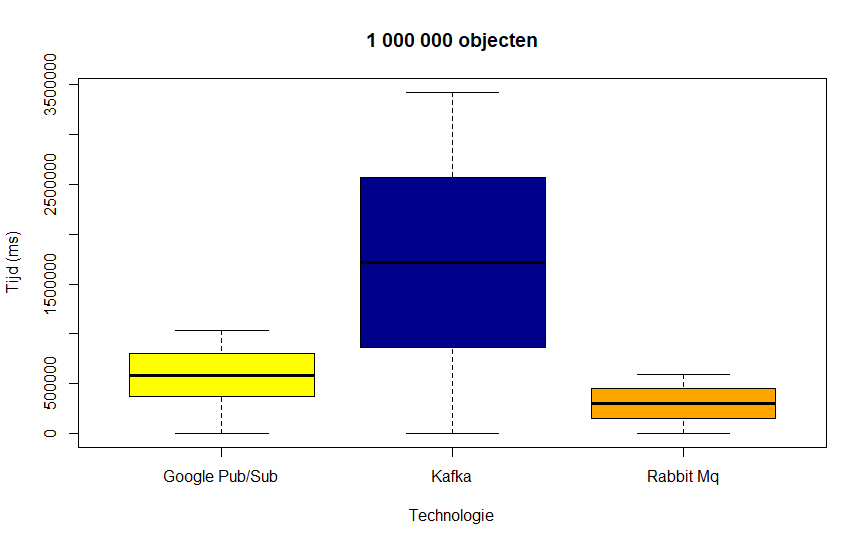
\includegraphics[width=100mm]{../1000000Boxplot.png}
    \caption{Vergelijking bij 1 000 000 objecten}
    
\end{figure}

Nu is het wat moeilijker om de snelheden met elkaar te gaan vergelijken aangezien de drie verschillende technologiëen verschillend aantal objecten hebben ontvangen. Toch overlopen we de technologieën eens.

Eerst gaan we de minimum waarden bekijken, hier kunnen we nog alle drie met elkaar vergelijken. Daarin is te zien dat RabbitMq nog steeds de kortste tijd heeft van de drie minimum waarden. Deze waarde is wel gestegen naar iets boven de seconde, maar blijft nog steeds de beste. Kafka is voor het eerst ook opvallend gestegen. De waarde is bijna vier keer zo groot geworden. Bij Google Pub/Sub zien we ook een stijging, het minimum ligt nu ook rond de drie seconden. Kafka heeft dus bij deze hoeveelheid het meeste tijd nodig als minimum waarde. 

Laat ons nu kijken naar de maximum tijd. Dit is wat moeilijker om te vergelijken aangezien al de technologieën verschillend aantal objecten ontvangen hebben. Kafka heeft het meeste tijd nodig, maar heeft ook het meeste objecten ontvangen. RabbitMq en Google Pub/Sub hebben ongeveer evenveel ontvangen, en daar zien we RabbitMq toch duidelijk beter zijn voor de maximum waarde.

Het resultaat van de maxima weerspiegelt zich ook opnieuw in de gemiddeldes. De verhoudingen zijn hetzelfde als bij de maximum waardes

Conclusie bij 1 000 000 objecten: RabbitMq doet het beter dan Google Pub/Sub. Kafka is moeilijk te vergelijken met de twee andere.

\subsection{Conclusie snelheid}
Op het gebied van snelheid is Kafka over het algemeen gezien de slechtste. Google Pub/Sub doet het over het algemeen gezien het beste, behalve bij super veel objecten (hier: 1 000 000) doet RabbitMq beter dan Google Pub/Sub.

\section{Memory}
\subsection{1 000 objecten}
Omdat de operatie om aan de Java runtime de gebruikte memory te vragen te lang duurt, wordt er enkel gekeken bij 1 000 objecten. Er wordt hier geen rekening gehouden met de snelheden.
\subsection{Conclusie memory}

Op figuur 5.4 ziet u de boxplots van het resultaat van het memory gebruik. Het is duidelijk te zien dat er bij alle technologieën enkele uitschieters zijn. Maar het is ook duidelijk dat over het algemeen voor het memory gebruik RabbitMq beter is. Het gemiddelde, maximum en het minimum liggen lager in vergelijking met de andere. Gemiddeld heeft RabbitMq 33.138 MB nodig. Google Pub/Sub en Kafka hebben gemiddeld 36.31 en 33.601 nodig. RabbitMq is dus beter maar het verschil met Kafka is klein. Het is enkel Google Pub/Sub die veel meer memory nodig heeft dan de rest.
\begin{figure}[h!]
    \centering
    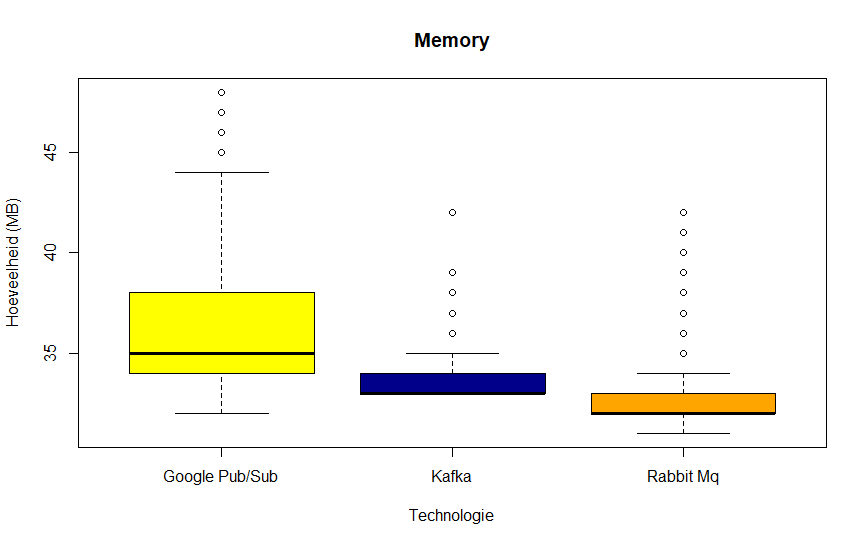
\includegraphics[width=100mm]{../memory.png}
    \caption{Vergelijking memory}
    
\end{figure}




%%=============================================================================
%% Bijlagen
%%=============================================================================

\appendix

%%---------- Onderzoeksvoorstel -----------------------------------------------

\chapter{Onderzoeksvoorstel}

Het onderwerp van deze bachelorproef is gebaseerd op een onderzoeksvoorstel dat vooraf werd beoordeeld door de promotor. Dat voorstel is opgenomen in deze bijlage.

% Verwijzing naar het bestand met de inhoud van het onderzoeksvoorstel
%---------- Inleiding ---------------------------------------------------------

\section{Introductie} % The \section*{} command stops section numbering
\label{sec:introductie}
Binnen TVH is er dus heel wat input van data die via microservices naar de juiste componenten verstuurd worden. Het spreekt voor zich dat niet ieder component, alle data nodig heeft. Daarom maakt dit bedrijf voornamelijk gebruik van de technologie \emph{Kafka} om met deze microservices te werken. Dit onderzoek zal nagaan of \emph{Kafka} inderdaad wel de beste technologie is om al deze data te verwerken in dit bedrijf. Aan de hand van deze onderzoeksvraag en deelvragen komt dit onderzoek hopelijk tot een besluit welke technologie het meest geschikt is:
\begin{itemize}
    \item Welke technologie is het best om met microservices te werken voor het bedrijf TVH?
    \begin{itemize}
        \item Bestaan er nog alternatieven voor \emph{Kafka} en \emph{RabbitMq}?
        \item Wat zijn de bevindingen van gebruikers?
        \item Welke technologie is het snelst?
    \end{itemize}
\end{itemize}


%---------- Stand van zaken ---------------------------------------------------

\section{Literatuurstudie}
\label{sec:Literatuurstudie}
In het onderzoek van \textcite{Shadija2017} staat te lezen dat microservices de business analysts helpen om grote schaalbare applicaties te maken. Het grote voordeel hiervan is flexibiliteit. Als er nieuwe functionaliteiten moeten worden gemaakt dan is het door de microservices gemakkelijk te implementeren. Vooral in het Internet of Things (IoT) domein kan dit het werk versoepelen. Dus voor het bedrijf TVH lijkt het de meest geschikte manier om de input van al de verzamelde data te verwerken.

Ook in andere onderzoeken naar microservices wordt \emph{Kafka} gebruikt. Zoals in het onderzoek van \textcite{Khazaei2017}. Als we kijken naar de conclusie uit dit onderzoek, blijkt dat \emph{Kafka} in grote lijnen het best scoort. De andere technologieën die in dit onderzoek gebruikt werden zijn \emph{Spark} en \emph{Cassandra}.

Het verschil van deze bachelorproef-onderzoek met het onderzoek van \textcite{Shadija2017} en het dat van \textcite{Khazaei2017} is dat dit onderzoek nagaat welke technologie het beste is voor het bedrijf TVH. Het besluit van dit onderzoek is dus niet noodzakelijk een algemeen besluit voor alle bedrijven die met microservices werken. Het onderzoek van \textcite{Khazaei2017} sluit hier het dichtst bij aan omdat het ook \emph{Kafka} en andere technologiën vergelijkt, maar het onderzoek legt meer de nadruk hoe flexibel een programmeerbaar, zelf-besturend IoT-platform is, gebruik makend van microservices. Het vergelijken van verschillende technologieën bij \textcite{Khazaei2017} is dus maar een klein onderdeel van het onderzoek en wordt bovendien in een andere architectuur toegepast zoals de titel meedeelt: `\emph{SAVI-IoT: A Self-Managing Containerized IoT Platform}`. De meerwaarde van deze vergelijking voor de conclusie is dus niet zo groot voor \textcite{Khazaei2017}.

Ook \textcite{Nycander2015} en \textcite{Cherradi2017} behandelen microservices in hun onderzoek.


% Voor literatuurverwijzingen zijn er twee belangrijke commando's:
% \autocite{KEY} => (Auteur, jaartal) Gebruik dit als de naam van de auteur
%   geen onderdeel is van de zin.
% \textcite{KEY} => Auteur (jaartal)  Gebruik dit als de auteursnaam wel een
%   functie heeft in de zin (bv. ``Uit onderzoek door Doll & Hill (1954) bleek
%   ...'')


%---------- Methodologie ------------------------------------------------------
\section{Methodologie}
\label{sec:methodologie}
Om te bepalen welke technologie het beste is bij het gebruiken van microservices, zal dit onderzoek de verschillende technologieën vergelijken. Eerst zal er een rondvraag gehouden worden over de bevindingen en de voor- en nadelen van \emph{Kafka} en \emph{RabbitMq}. Er wordt ook eens gepolst als mensen met nog andere technologieën reeds gewerkt hebben en wat daar de bevindingen zijn.

Dan zal er onderzocht worden als er effectief nog alternatieven bestaan voor \emph{Kafka} en \emph{RabbitMq}.

Als laatste zal op een virtuele machine de realiteit nagebootst worden. Dit wordt gedaan door elke technologie op deze virtuele machine te zetten en daarna te gaan meten wat de snelheden zijn bij het opvragen, verwerken, ... van voorbeelddata.

%---------- Verwachte resultaten ----------------------------------------------
\section{Verwachte resultaten}
\label{sec:verwachte_resultaten}
Het resultaat van dit onderzoek zal hopelijk aanwijzen welke technologie het meest geschikt is voor deze hoeveelheid van data aan te kunnen. We hopen dit te zien door cijfergegevens van de snelheden van uitvoering. 


%---------- Verwachte conclusies ----------------------------------------------
\section{Verwachte conclusies}
\label{sec:verwachte_conclusies}

Aangezien TVH al gebruik maakt van \emph{Kafka}, en ook in andere onderzoeken \emph{Kafka} gebruikt werd of bestempeld werd als beste oplossing, kunnen we in dit onderzoek hopelijk ook concluderen dat \emph{Kafka} de beste oplossing is om met microservices om te gaan.



%%---------- Andere bijlagen --------------------------------------------------
% TODO: Voeg hier eventuele andere bijlagen toe
%\input{...}

%%---------- Referentielijst --------------------------------------------------

\printbibliography[heading=bibintoc]
%\addcontentsline{toc}{chapter}{\textcolor{maincolor}{\IfLanguageName{dutch}{Bibliografie}{Bibliography}}}

\end{document}
